% Options for packages loaded elsewhere
\PassOptionsToPackage{unicode}{hyperref}
\PassOptionsToPackage{hyphens}{url}
\PassOptionsToPackage{dvipsnames,svgnames,x11names}{xcolor}
%
\documentclass[
  letterpaper,
  DIV=11,
  numbers=noendperiod]{scrartcl}

\usepackage{amsmath,amssymb}
\usepackage{iftex}
\ifPDFTeX
  \usepackage[T1]{fontenc}
  \usepackage[utf8]{inputenc}
  \usepackage{textcomp} % provide euro and other symbols
\else % if luatex or xetex
  \usepackage{unicode-math}
  \defaultfontfeatures{Scale=MatchLowercase}
  \defaultfontfeatures[\rmfamily]{Ligatures=TeX,Scale=1}
\fi
\usepackage{lmodern}
\ifPDFTeX\else  
    % xetex/luatex font selection
\fi
% Use upquote if available, for straight quotes in verbatim environments
\IfFileExists{upquote.sty}{\usepackage{upquote}}{}
\IfFileExists{microtype.sty}{% use microtype if available
  \usepackage[]{microtype}
  \UseMicrotypeSet[protrusion]{basicmath} % disable protrusion for tt fonts
}{}
\makeatletter
\@ifundefined{KOMAClassName}{% if non-KOMA class
  \IfFileExists{parskip.sty}{%
    \usepackage{parskip}
  }{% else
    \setlength{\parindent}{0pt}
    \setlength{\parskip}{6pt plus 2pt minus 1pt}}
}{% if KOMA class
  \KOMAoptions{parskip=half}}
\makeatother
\usepackage{xcolor}
\setlength{\emergencystretch}{3em} % prevent overfull lines
\setcounter{secnumdepth}{-\maxdimen} % remove section numbering
% Make \paragraph and \subparagraph free-standing
\ifx\paragraph\undefined\else
  \let\oldparagraph\paragraph
  \renewcommand{\paragraph}[1]{\oldparagraph{#1}\mbox{}}
\fi
\ifx\subparagraph\undefined\else
  \let\oldsubparagraph\subparagraph
  \renewcommand{\subparagraph}[1]{\oldsubparagraph{#1}\mbox{}}
\fi


\providecommand{\tightlist}{%
  \setlength{\itemsep}{0pt}\setlength{\parskip}{0pt}}\usepackage{longtable,booktabs,array}
\usepackage{calc} % for calculating minipage widths
% Correct order of tables after \paragraph or \subparagraph
\usepackage{etoolbox}
\makeatletter
\patchcmd\longtable{\par}{\if@noskipsec\mbox{}\fi\par}{}{}
\makeatother
% Allow footnotes in longtable head/foot
\IfFileExists{footnotehyper.sty}{\usepackage{footnotehyper}}{\usepackage{footnote}}
\makesavenoteenv{longtable}
\usepackage{graphicx}
\makeatletter
\def\maxwidth{\ifdim\Gin@nat@width>\linewidth\linewidth\else\Gin@nat@width\fi}
\def\maxheight{\ifdim\Gin@nat@height>\textheight\textheight\else\Gin@nat@height\fi}
\makeatother
% Scale images if necessary, so that they will not overflow the page
% margins by default, and it is still possible to overwrite the defaults
% using explicit options in \includegraphics[width, height, ...]{}
\setkeys{Gin}{width=\maxwidth,height=\maxheight,keepaspectratio}
% Set default figure placement to htbp
\makeatletter
\def\fps@figure{htbp}
\makeatother

\KOMAoption{captions}{tableheading,figureheading}
\makeatletter
\makeatother
\makeatletter
\makeatother
\makeatletter
\@ifpackageloaded{caption}{}{\usepackage{caption}}
\AtBeginDocument{%
\ifdefined\contentsname
  \renewcommand*\contentsname{Tabla de contenidos}
\else
  \newcommand\contentsname{Tabla de contenidos}
\fi
\ifdefined\listfigurename
  \renewcommand*\listfigurename{Listado de Figuras}
\else
  \newcommand\listfigurename{Listado de Figuras}
\fi
\ifdefined\listtablename
  \renewcommand*\listtablename{Listado de Tablas}
\else
  \newcommand\listtablename{Listado de Tablas}
\fi
\ifdefined\figurename
  \renewcommand*\figurename{Figura}
\else
  \newcommand\figurename{Figura}
\fi
\ifdefined\tablename
  \renewcommand*\tablename{Tabla}
\else
  \newcommand\tablename{Tabla}
\fi
}
\@ifpackageloaded{float}{}{\usepackage{float}}
\floatstyle{ruled}
\@ifundefined{c@chapter}{\newfloat{codelisting}{h}{lop}}{\newfloat{codelisting}{h}{lop}[chapter]}
\floatname{codelisting}{Listado}
\newcommand*\listoflistings{\listof{codelisting}{Listado de Listados}}
\makeatother
\makeatletter
\@ifpackageloaded{caption}{}{\usepackage{caption}}
\@ifpackageloaded{subcaption}{}{\usepackage{subcaption}}
\makeatother
\makeatletter
\@ifpackageloaded{tcolorbox}{}{\usepackage[skins,breakable]{tcolorbox}}
\makeatother
\makeatletter
\@ifundefined{shadecolor}{\definecolor{shadecolor}{rgb}{.97, .97, .97}}
\makeatother
\makeatletter
\makeatother
\makeatletter
\makeatother
\ifLuaTeX
\usepackage[bidi=basic]{babel}
\else
\usepackage[bidi=default]{babel}
\fi
\babelprovide[main,import]{spanish}
% get rid of language-specific shorthands (see #6817):
\let\LanguageShortHands\languageshorthands
\def\languageshorthands#1{}
\ifLuaTeX
  \usepackage{selnolig}  % disable illegal ligatures
\fi
\usepackage[]{biblatex}
\addbibresource{../../../../references.bib}
\IfFileExists{bookmark.sty}{\usepackage{bookmark}}{\usepackage{hyperref}}
\IfFileExists{xurl.sty}{\usepackage{xurl}}{} % add URL line breaks if available
\urlstyle{same} % disable monospaced font for URLs
\hypersetup{
  pdftitle={La Economía Agraria},
  pdfauthor={Achalma Mendoza Edison},
  pdflang={es},
  colorlinks=true,
  linkcolor={blue},
  filecolor={Maroon},
  citecolor={Blue},
  urlcolor={Blue},
  pdfcreator={LaTeX via pandoc}}

\title{La Economía Agraria\thanks{gracias}}
\usepackage{etoolbox}
\makeatletter
\providecommand{\subtitle}[1]{% add subtitle to \maketitle
  \apptocmd{\@title}{\par {\large #1 \par}}{}{}
}
\makeatother
\subtitle{Una leccion detallada de economia agraria}
\author{Achalma Mendoza Edison}
\date{2022-04-22}

\begin{document}
\maketitle
\begin{abstract}
hola
\end{abstract}
\ifdefined\Shaded\renewenvironment{Shaded}{\begin{tcolorbox}[frame hidden, breakable, sharp corners, interior hidden, borderline west={3pt}{0pt}{shadecolor}, boxrule=0pt, enhanced]}{\end{tcolorbox}}\fi

\hypertarget{econompia-agraria-y-rural}{%
\section{Econompia agraria y rural}\label{econompia-agraria-y-rural}}

\hypertarget{la-economuxeda-agraria}{%
\subsection{La economía agraria}\label{la-economuxeda-agraria}}

En sus inicios aplicó los principios de la agricultura van juntamente
con la ganadería, que posteriormente es como una disciplina científica
que se ocupó muy primitivamente, al convertirse en las necesidades de
mejorar los rendimientos y la productividad se ocupó del uso de la
tierra y los métodos para optimizar para la toma de decisiones de los
productores agropecuarios.

Se presentan tres áreas:

\begin{itemize}
\item
  El uso de la tierra (identificación del recurso tierra)
\item
  Los métodos usados para el uso de la tierra (herramienta o técnica que
  se usa)
\item
  La toma de decisiones (del productor agropecuario, agronegocios)
\end{itemize}

\textbf{Adam Smith:} consideró que la tierra como bien escaso genera una
renta semejante a la de todo monopolio.

\textbf{David Ricardo:} que la renta es la porción del producto de la
tierra que se paga al propietario por el uso de ``las fuerzas
originarias'' del suelo y por tanto varía según la calidad y ubicación
del terreno.

\textbf{Carlos Marx:} optó por distinguir entre la ``renta absoluta''
que resulta de la concentración de la propiedad de la tierra y la
``renta diferencial''.

\textbf{Henry Charles Carey:} Cuestionó las tesis de Smith y Ricardo
sobre la renta en cuanto que consideró que siempre habría disponibles
tierras de calidad y tecnología que permitiera producir más. La
alternativa al modelo europeo, el modelo estadounidense de tierras
disponibles y proteccionismo

\textbf{Johann Heinrich Von Thünen:} hizo un aporte decisivo a la
economía agrícola con su teoría de la localización, basada en el
supuesto según el cual, si la actividad agrícola se pudiese concentrar,
como la producción industrial se situaría cerca del mercado, enfatizando
la importancia de la renta de localización, que, sin negar otros
factores, postulaba como elemento más importante para configurar el
territorio agropecuario.

Hoy el estudio de la geografía rural tiene en cuenta por una parte que
una nueva ruralidad ha determinado la importancia de actividades no
agropecuarias en el campo, como la minería y otras extractivas.

\hypertarget{teorema-de-la-telarauxf1a}{%
\subsection{Teorema de la telaraña}\label{teorema-de-la-telarauxf1a}}

Muestra la relación con la determinación del equilibrio en aquellos
casos en que los ajustes son completamente discontinuos. Un campo de la
economía agropecuaria es el de la especificidad de los mercados del
sector. Al principio simplemente se estudió la aplicación de la oferta y
demanda.

Según alexander chayanov: quien estudió la especificidad de la economía
campesina, la organización de la unidad productiva familiar: sus
objetivos y planes, la circulación de capital, trabajo y familia; las
consecuencias de todo ello para la economía nacional e internacional y
la articulación de la economía campesina con el conjunto económico.
Contribuye a revalorar el aporte de los campesinos a la economía y
explicar la heterogeneidad de las formas de producción agropecuarias
contemporáneas. En uno de los libros menciona que el campesino tiene
ventaja frente a otros, pero basado en la URSS (Socialismo) y defendía a
la economía campesina.

\hypertarget{escala-de-producciuxf3n}{%
\subsection{Escala de producción}\label{escala-de-producciuxf3n}}

Los economistas aplicaron los postulados clásicos de economía de escala
al sector agropecuario para predecir el triunfo de la gran producción en
el sector, como en el resto de la economía, tan sólo limitada por la ley
de los rendimientos decrecientes, o sea por la proporcionalidad en el
incremento de los distintos factores productivos (en algún momento va a
llegar a un punto de saturación y va a decrecer la producción)

\textbf{Jacob Viner:} concibió la agricultura campesina como uno de los
factores de atraso que generan pobreza (mantener al campesino en esa
condición es condenarla a la pobreza continua o sea a las siguientes
generaciones). Viner comienza a notar sin mencionar como los efectos de
la economía externa (capitalista) comienza a afectar a la economía
campesina porque no se adapta a las exigencias del mercado por lo que
estará condenado a la pobreza permanente.

\textbf{Vandana Shiva:} ha cuestionado todo el modelo de gran producción
agropecuaria y el cambio tecnológico que lo ha acompañado, la revolución
verde y ha contabilizado los costos ambientales y otros costos no
pagados por los agronegocios, que al permitir el consumo gratuito de
recursos garantizan una rentabilidad privada a costa de un enorme costo
social e impacto ambiental.

La agronomía, también nombrada ingeniería agronómica, es la agrupación
de conocimientos de múltiples disciplinas que dirigen la praxis de la
agricultura y la ganadería.

El objetivo de la ingeniería en agronomía es conseguir una mejora en la
calidad de las técnicas de la producción y el proceso de transformación
de artículos alimentarios y agrícolas basándose tanto en fundamentos
tecnológicos como en científicos y a través del examen de los factores
biológicos, físicos, económicos, químicos y sociales que intervienen o
perjudican el desarrollo productivo. El propósito de estudio de la
agronomía es la transformación social del agroecosistema.

El problema económico se puede definir con dos afirmaciones corrientes

\begin{itemize}
\tightlist
\item
  En la que nosotros como economistas estamos enfrentados a las
  finalidades múltiples en competencia entre los que se debe de elegir
  en tal elección se debe renunciar a otras alternativas deseables
  (costo de oportunidad). Uno no puede ordeñar la vaca y al mismo tiempo
  venderla.
\item
  No se puede obtener algo por nada, toda acción hacia la obtención de
  algo implica sacrificar algo, es decir, tiene un costo. No hay
  almuerzo gratis.

  \begin{itemize}
  \tightlist
  \item
    Los recursos abundantes, que pueden obtenerse sin esfuerzo alguno,
    son bienes no económicos o libres, o gratuitos. Aquellos que son
    obtenidos con el esfuerzo humano, son bienes económicos. Que todo
    tiene un precio o un costo
  \item
    La búsqueda o consecución de estos últimos para satisfacer
    necesidades es lo que da origen a actos económicos. Y el
    encadenamiento y repetición sistemática de dichos actos es a lo que
    se le llama actividad económica. Aquí está la habilidad, la
    formación del profesional en economía para determinar las acciones
    correctas que se deben de ejecutar para satisfacer necesidades desde
    elegir el terreno hasta llegar al mercado (es encadenado).
  \item
    La enorme cantidad de bienes que la sociedad utiliza pueden
    clasificarse desde dos ángulos:
  \end{itemize}
\end{itemize}

Según su naturaleza y según su función

\textbf{Según su naturaleza,} los bienes pueden entenderse:

\begin{enumerate}
\def\labelenumi{\arabic{enumi}.}
\item
  Como el modo de ser de los mismos vistos con referencia al ser humano;
  pueden ser naturales, es decir no son producidos por los humanos; es
  decir, los seres humanos y sus facultades; y manufacturados, producto
  de la combinación de la acción de los seres humanos y los recursos
  naturales
\item
  Como la manera de ser de los bienes considerados en sí mismos. Con
  referencia a la manera de ser de los bienes, pueden ser materiales, o
  sea, con existencia física e inmateriales, o sea pueden ser productos
  de la mente (tiene mayor valor)
\end{enumerate}

\textbf{Según su función,} los bienes pueden verse como:

\begin{enumerate}
\def\labelenumi{\arabic{enumi}.}
\item
  Bienes directos, o de consumo, son aquellos que se destinan al
  disfrute inmediato. El aire y la luz solar, un paisaje natural, una
  fruta comestible, por ejemplo, son de este tipo en la medida en que
  satisfacen la necesidad de respirar, de obtener energía, de
  recreación, de alimentación, etc.
\item
  Bienes indirectos, llamados también factores de producción, los cuales
  se emplean en preparar la satisfacción de las necesidades, mediante la
  obtención, con ayuda de ellos, de otros que de modo directo la
  satisfacen: la lluvia, la energía solar, los minerales del suelo, la
  mano de obra, las máquinas y equipos, son de este tipo, en la medida
  en que ayudan a producir otros bienes.
\end{enumerate}

Entonces si ya sabemos sobre recursos, elección, objetivos múltiples, y
la idea de escasez, se puede definir la naturaleza y el alcance del
campo de la Economía como: la Ciencia social que trata cómo los
individuos, las empresas, el Estado y otras entidades de la sociedad
asignan recursos en el marco de una situación de escasez caracterizada
por el enfrentamiento de objetivos alternativos (es una definición de la
economía).

Entonces la economía agraria implica la aplicación de la Economía a la
agricultura; por lo tanto, se puede definir el campo de la Economía
Agraria como Una Ciencia social aplicada que trata sobre cómo los
productores, los consumidores y la sociedad usan los recursos escasos en
la producción. procesamiento mercadeo y consumo de productos
alimenticios y fibras. (no se estudia a la producción en sí sino
analizar todo lo que hace el agricultor como y donde produce y vemos
nosotros para quien produce (mercadeo es el más importante que la
producción).

Es una actividad del ser humano llevada a cabo para producir alimentos y
fibras (lana, seda, algodón) mediante el uso deliberado (no cualquiera
lo hace) y controlado de vegetales y animales.

\hypertarget{economuxeda-rural}{%
\subsection{Economía rural}\label{economuxeda-rural}}

Tiene un objeto estudio más amplio que la economía agraria porque supera
la visión de trabajo del sector, además que la unidad elemental de
análisis ya viene a ser él hogar del trabajador. Se analiza las fuentes
de ingreso de la familia rural o del hogar. La economía rural fue
recientemente más o menos hace 30 o 40 años ha empezado a desarrollarse
debido a la gran heterogeneidad social de la población rural o de los
habitantes de las zonas rurales.

Influencia del lugar:

\begin{itemize}
\item
  \textbf{Sierra:} probablemente sea mucho más itinerante. Pero si son
  cultivos que cosechan una vez al año, entonces los padres van a salir
  de ella para tratar de obtener ingresos por otras actividades que no
  son la actividad agraria. La migración de la fuerza de trabajo de los
  padres de familia del hogar, pueden ser prolongados. El poblador rural
  además de su actividad agropecuaria puede ser un comerciante puede ser
  un artesano o puede salir a la ciudad a ofrecer sus servicios o de
  repente ofrece servicios de transporte de carga y son varias las
  fuentes de ingreso que va a obtener para el bienestar de su hogar.
\item
  \textbf{Costa:} puede ser mucho más sedentario porque las fuentes de
  ingresos son diversos en los hogares según incluso tipos de cultivo
  que si son cultivos permanentes el lugar va a ser mucho más estable,
  no se va a mover mucho siempre va a estar el lugar más íntegro.
\end{itemize}

Además de incorporar en este análisis, el surgimiento o la aparición y
el desempeño de las instituciones agrarias tanto privadas como públicas
la economía rural influye en la participación de organismos públicos.
que acuden en su apoyo o puede y no colabora con actividad que
normalmente ocurre, por ejemplo, con la Dirección Regional Agraria se
limita a entregar mangueras a enviar un par de técnicos agropecuarios a
ver.

\hypertarget{quuxe9-es-economuxeda-rural}{%
\subsubsection{¿Qué es economía
rural?}\label{quuxe9-es-economuxeda-rural}}

La economía rural, tiene un concepto más amplio del sector, porque ya la
unidad de análisis ya viene ser el hogar del trabajador en el área
rural, como un subconjunto de la actividad económica, pero no deja de
analizar la economía agraria, incorpora el comportamiento y cuáles son
los ingresos del área rural. Ha empezado a desarrollarse gracias a la
heterogeneidad, un comportamiento diferente según su grado de
influencia, en el ambiente en el cual se desenvuelven, en la sierra
itinerante, costa más sedentaria, porque los ingresos varían, según el
tipo de cultivos, si rotan rápidamente, o solo si es una cosecha al año,
los padres salen para obtener más ingresos, para su bienestar familiar.
De modo que el hogar se fracciona. La economía rural incorpora el
comportamiento, el quehacer diario y las fuentes de ingreso de la
familia rural. Fuentes de ingreso, tamaño de la tierra. Analizamos al
actor principal que es el hombre, la pobreza, la transferencia del área
rural al área urbano. Educación del poblador. Análisis de derechos
humanos.

\begin{itemize}
\item
  Ingreso obtenido por los habitantes en la zona rural en las diversas
  actividades ejerce.
\item
  Consideramos cómo es que la pobreza y la desigualdad son indicadores
  casi universales para gran parte de la población.
\item
  Relacionar los ingresos y la falta o la seguridad alimenticia que hay
  en el área rural como parte de la pobreza y la desigualdad.
\item
  El acceso a bienes y servicios públicos como la salud y la educación
  hasta qué punto es cercano al poblador rural.
\item
  Como efecto de la falta de salubridad en su alimentación o la falta de
  educación, desnutrición, anemia.
\item
  La economía rural ha empezado a desarrollarse debido a la gran
  heterogeneidad social, comportamiento diferente según el grado de
  influencia de acuerdo con el ambiente en el cual se desenvuelve.
\item
  Las fuentes de ingreso son diversas, según tipo de cultivo.
\item
  El hogar será más estable e íntegro, pero si son cultivos que rotan
  rápidamente y si es cosecha solo 1 vez al año, trataran de cambiar
\item
  Múltiples determinantes de bienestar van a influir, la migración de
  fuerzas de trabajo será prolongados hasta ejercer la actividad rural
\item
  Tal Vez con un poco más de detenimiento, economía rural lo hubiéramos
  llamado así
\item
  Las diferentes fuentes de ingreso del trabajador del área rural.
\item
  Procesamiento
\item
  Mercadeo
\item
  Consumo
\item
  De la actividad agraria
\item
  Factor hombre
\item
  Además de agricultor, puede ser comerciante u hacer otra actividad.
\end{itemize}

\hypertarget{la-economuxeda-agraria-1}{%
\subsection{La economía agraria}\label{la-economuxeda-agraria-1}}

Es un acto deliberado controlado de los vegetales y animales, un poco
juntando sería pecuario, sería Agropecuario. Esferas de la producción,
el mercadeo, solamente agropecuario.

Manejo el forestal por eso se amplía su aspecto, porque su campo de
acción de amplia \textbf{aún es restringido porque no considera el
análisis del agricultor, allí ingresa el concepto de economía rural}.

\hypertarget{quuxe9-es-la-actividad-agraria}{%
\subsubsection{¿Qué es la actividad
agraria?}\label{quuxe9-es-la-actividad-agraria}}

En la actividad agraria nos referimos solo al sectorial los productores
y consumidores, procesamiento y mercadeo, pero de la actividad agraria,
no incluimos a la actividad hombre.

\textbf{¿Cómo es que la pobreza y la desigualdad son indicadores?}

Los ingresos que son bajos ponen en riesgo la seguridad alimentaria que
debe tener la población, pero no cuentan con los recursos para
satisfacer sus necesidades básicas.

O esperamos sentados en nuestros escritorios, la educación se vuelva en
igualdad de condiciones, ya sería suficiente, la equidad es totalmente
distinta, la calidad de vida se tiene que analizar. Castillo dijo que
enviaría un médico por cada habitante, entonces sería un gran avance,
para que se desenvuelva en igualdad de condiciones, la equidad del
poblador rural es totalmente distinta, la calidad de vida hay que
caracterizar con la lupa de la caracterización\textbf{.}

\textbf{¿Cuáles son las enfermedades comunes, efecto de la mala
alimentación y de educación, generando mayores niveles de desnutrición,
de anemia, porque no tiene los hábitos suficientes de higiene?}

Atreves de la afección intestinal, lo va a votar, de que las capacidades
deben ser mayores en el área rural. En relación con el área urbana, hay
área rural donde más prima las diferencias. En cuanto a la ley sobre
derechos urbanos, no se debe generar expectativas que no existen, deben
considerar más que solo tienen derechos y no obligaciones, ellos estaban
haciendo la minería, más conocen sus derechos que sus deberes.

Derechos de territorio, las tierras de minería, esa era nuestra chacra y
allí vivíamos, deberíamos incorporar en el análisis rural, que influyen
al sector agrario y cuanto dependen de la agricultura y cuanto de la
minería.

Los derechos humanos bien entendidos, deberían incorporar las
obligaciones.

\textbf{La economía rural es más grande que la economía agraria.}

Porque en agraria solo se ve la producción y mercadeo de agropecuario,
en la rural se considera además de todo a la familia, allí tocamos los
niveles de ingreso, la elección o estrategia que toma para generar
fuentes de ingreso, la tierra, la pobreza, la desigualdad, transferencia
de riqueza, la calidad de vida del poblador, allí se ve la riqueza de
análisis, de derechos humanos en las comunidades.

Las direcciones Regionales Agrarias, tratan de implementar una economía
rural, sin embargo, su actividad es muy limitada, el enfoque no refleja
la necesidad del área rural, puedo decir que si mañana, a partir del día
de mañana no existe la DRAA, ¿afectaría a los productores agrarios en
algo?

Tal vez para trámites de certificación o para el registro de propiedad
en SUNARP. O lo sacamos de COFOPRI de catastro Rural, ya no lo llamamos,
de servicio de titulación de tierras de Ayacucho. No le afectaría mucho
al trabajador, tenemos una institución muy burocrática.

A veces más se le ponen obstáculos al agricultor. O mejor darlo al
campesino, la moto es para 5 años y le haga mantenimiento.

\begin{itemize}
\item
  Es bueno saber que la DRAA debe apoyar al sector agrario, los que van
  al rural o derecho de paso, o el pago por daño o desastres en realidad
  le llega a la gente que no le corresponde, y se queda con los
  funcionarios con DNI falsos.
\item
  Sería buena si es mejor diseñada y que realmente esté dirigido al
  AGRO, sobre la posición de necesidades, de traer información real, de
  acuerdo con ello crear estrategias. Se convirtió en un vaso envolvente
  o todo lo que llega a ese recipiente el 80\% se queda en la burocracia
  y solo el 20\% se le da a los afectados en la DRAA.
\item
  Un director regional, cómo obtiene la información estadística, saca
  una muestra, solo unas cuantas hectáreas.
\end{itemize}

\hypertarget{la-agricultura-y-el-desarrollo}{%
\section{La agricultura y el
desarrollo}\label{la-agricultura-y-el-desarrollo}}

En la actividad agropecuaria es importante el estudio de los efectos del
rápido crecimiento de la población, entendiendo que debe afectar al
desarrollo integral del país.

¿Qué consecuencias o cómo afecta el aumento de la población en el área
rural al conjunto de la economía?

En países en desarrollo se da una combinación de alta tasa de fertilidad
con bajas tasas de mortalidad.

Estas altas tasas de fertilidad significan que debe destinarse más
recursos naturales a la agricultura, solo para lograr satisfacer los
mismos requerimientos de alimentos. Por cabeza va a aumentar el grado de
satisfacción, asignando cada vez más recursos.

Si son 10 personas en el área rural y aumentan a 15 personas, para 10 a
un pan era ahora tendría que ser 15, y sigue considerándose un pan por
cabeza. Allí sí se mejoraría la condición de vida del poblador rural.
Esto pone en desventaja frente al área urbana. El crecimiento
demográfico es mayor en el área urbana. Sacrifica más recursos, menor
calidad vida, menores ingresos, pese a que se puede atender con más
recursos.

El crecimiento rápido disminuye el crecimiento global de la economía.

Debemos decidir eficientemente ¿cuál inversión? ¿Cuáles son las
prioridades y en qué condiciones se va a determinar estos rendimientos o
crecimiento? ¿Inversiones Estratégicas?

\begin{itemize}
\item
  En la década de los 90, se implementó una política de control de
  natalidad a la mujer que tiene muchos hijos se les ligó (Ligadura,
  vasectomía).
\item
  A los 28 ya tenía 6, su nivel de ingreso era bajo, y tenía 6 hijos,
  sacrificando 6 vidas para el futuro.
\item
  Y lo que paso que solo tenían 1 hijo y lo ligaron, allí las enfermeras
  y los médicos tenían que cumplir metas para que sea efectivo
\item
  En el área urbana, se quedan con sus hijos. Hay un control la
  población está aprendiendo
\item
  Ahora crecemos a 1\%, ya hay un control. Tomar en cuenta la
  información femenina y masculina, los nacimientos por año. Los
  nacimientos por día.
\item
  Los médicos tienen que elegir entre una mamá y un hijo. Y salvan a la
  mama.
\item
  El sector salud se está relajando, arrinconamiento de la actividad.
  Cuántos van del área urbana al área rural
\end{itemize}

Crecimiento poblacional de Ayacucho

Migración del campo a la ciudad, si esto afecta en el pbi de Ayacucho

Población y producción

El valor de la producción y migración

\textbf{Palta}

Plantones trajeron de Ica, y están produciendo 4000 toneladas de paltos.

100 platos es una yugada, pueden sacar 2 toneladas a 3 toneladas de
palta 5000 dólares -- 18 mil dólares por año

Manejo técnico

Gestión pública he estado, recién empezó como docente y producir

Abono foliar

Grupo de contenedores lo han devuelto al Perú

Mi hermana tiene 25 hectáreas de paltos, elegir al exportador, un
empresario grande

Fumigar con insecticida, Mario esta bonito, agarramos planta por planta
hizo sacar mi hermano, 360 plantones, no ven a un agricultor en su zona,
aprenden con el ejemplo y demostrar, si se puede o no.

Había una hectárea de palta que se malogro, por mucha insecticida y él
lo eliminó todo para que no contagie a los demás.

El uso de agua en la producción de palto, si ahora estás preocupado en
la producción de agua o siembras palto.

Cuando los pobladores no ven un agricultor exitoso, entonces solo
aprenden con el ejemplo. El agua es un problema fundamental. Chile ya no
tenía agua para su consumo, por el sembrío. En Chile están con la
regionalización de la población. Preocupación del uso de agua.
Aprovechas ahora y siembras palto sin importar.

Los noticieros sacan informes completos de Alemania, Francia,
información convincente, manejar más información debería ser, hablando
de desecho de animales. Un producto que estaba prohibido hace 5 años,
pero un grupo nos querían vender a nosotros, Perú fumiga anualmente. Yo
lo dejé así, y en el comercio salió una noticia y hablaban de que
podríamos fumigar por muchas razones y tenemos una conferencia de medio
ambiente. Y no siguió porque era tóxico.

\hypertarget{problema-de-la-poblaciuxf3n-para-el-sector-agruxedcola}{%
\subsection{Problema de la población para el sector
agrícola}\label{problema-de-la-poblaciuxf3n-para-el-sector-agruxedcola}}

Es explicado en términos de tasa de crecimiento en su número o en su
densidad, cuan disperso es para ver lo que el área urbana le puede
brindar. En promedio en Ayacucho, el tamaño de la tierra es 0.75 por
persona, el problema fundamental del agro es el tamaño de la tierra.

Entonces no es un problema como dijo Malthus, la gente geométricamente y
la comida aritméticamente, ver la densidad. En mayor porcentaje creció
la producción mundial y los ingresos, conforme lo que tenemos un
problema de distribución porque el incremento del ingreso y de la
producción creció en la zona urbana en las ciudades y los precios si
regulan los precios en el consumo, en países como el nuestro, tendremos
problemas en la producción.

No permite una inversión de capital, en el LP, podría reivindicarse a
Malthus, de aquí a muchos años cuando estemos saturados, tal vez
tengamos mucha población y no haya tierras para la actividad
agropecuaria.

El problema de la población de aquí 100 años, tenemos más personas en el
mundo y no tenemos tierra para la actividad agropecuaria, de repente con
una pastilla comemos todo, tenemos problema de distribución, dado la
población que está dedicada a la actividad agropecuaria.

El petróleo es el más contaminante de lo que sacan del petróleo y nos
inundaron a todo el mundo con contaminación, los grandes intereses que
existe en el mundo. Y los agricultores solo tienen sus vacas y dicen que
prefieren tener y porque no cierran a esas grandes empresas que generan
más, como cuando extraen petróleo.

Sin crecimiento no hay desarrollo, desarrollo si necesita de
crecimiento.

Podemos decir que el desarrollo significa crear condiciones para la
racionalización de la actividad peruana.

Desarrollo significa crear las condiciones para la realización de la
personalidad humana. Por tanto, es posible que un país alcance un
crecimiento económico, sin que alcance un nivel mayor de desarrollo.

Puede haber crecimiento, pero no desarrolló, puedo estar sembrando más,
pero no por eso se ha desarrollado la actividad, crece la disponibilidad
de recursos, pero eso no dice que hubo desarrollo, con la misma
extensión produzco más eso si es desarrollo, con maquinarias y equipo,
canales de distribución, más conocimiento, más educación.

Mano de obra oportuna, tal vez tienes escasez, pero fuera hay mano de
obra desempleada, a eso se le llama, desequilibrio laboral, los
trabajadores no están informados de las oportunidades de trabajo.
Podemos analizar la Oferta de Mano de Obra.

Palta

\begin{itemize}
\item
  Para la cosecha trae 20 trabajadores, yo tengo que ir a coger lo que
  dejan, con mis 3 o 4 trabajadores que tengo.
\item
  Quiero 10 y suben.
\item
  Mano de Obra siempre hay disponible no siempre en localidad sino
  fuera.
\item
  Desarrollo es más amplio que crecimiento económico.
\end{itemize}

Desarrollo significa crear condiciones las condiciones para la
realización humana, dirigido a la persona al grado de satisfacción,
puede que el país tenga crecimiento, pero no desarrollo, no es efecto
del incremento de la productividad, generalmente viene acompañado del
desarrollo y de la reducción de la pobreza, porque con el mismo tamaño
se produce más, podemos trabajar con mejor mano de obra, mejor tg, mejor
uso de recursos.

Ejemplo cuando está llena la olla, y se saca el agua con jarra hay
desperdicio de recursos.

Crecimiento económico es la realización de la personalidad humana es
posible considerar para su análisis, indicadores importantes que nos
puedan decir si hay cambios o no en el nivel de vida de la población.

\hypertarget{indicadores-de-pobreza}{%
\subsection{Indicadores de pobreza}\label{indicadores-de-pobreza}}

\begin{itemize}
\item
  \textbf{La PROPORCIÓN de las personas que viven debajo de algún nivel
  de pobreza definido.} 2\(x familia, debajo de 1.5\)X PERSONA está en
  extrema pobreza. Pobre es aquel para nosotros menor 3\$, tienen
  niveles de ingresos mucho más altos, pero se consideran pobres de
  acuerdo con lo mencionado, nivel de vida distinta.
\item
  \textbf{LA TASA DE DESEMPLEO:} Se tiene mucho desempleo, hay una gran
  cantidad de población que no tiene ingreso. Ejemplo: Ica tenía 0\% de
  desempleo, aun cuando el salario era 35 soles, todo el mes estaba
  ocupado el trabajador. En Ayacucho 40 soles, una semana al mes
  trabaja, esa mano de obra de Ica es más productiva. Chaqcha, comida,
  agua.
\item
  \textbf{LA DESIGUALDAD DEL INGRESO}: Cuán amplia es la diferencia del
  ingreso del pobre y el rico, cuando más amplia es la brecha, la
  pobreza es mayor. No es evitar que el rico que crezca más, pero esos
  ingresos se acerquen o aumente más, aun cuando se aleje, aumente en el
  mismo sentido, lo que genera es el empleo. Empresas de mandarina,
  paltos, etc.
\item
  \textbf{DESERCIÓN ESCOLAR,} No tendrán el mismo nivel de oportunidades
  de los que sí fueron a las universidades.
\item
  \textbf{DERECHOS CIVILES Y CONSTITUCIONALES:} Como ve su participación
  en los derechos civiles, conocen sus deberes.
\end{itemize}

Van a representar una mejora y para tener derechos cumplió con muchas de
sus obligaciones. Los servicios están a su alcance. Sabe que puede ir a
la Municipalidad y puedan poner alumbrado público, canal de riego.

\begin{itemize}
\item
  TASA DE DESEMPLEO
\item
  NIVELES DE INGRESO
\item
  AMPLITUD DE DESIGUALDAD
\item
  DERECHOS CIVILES INDIVIDUALES Y GRUPALES
\item
  JUSTICIA
\item
  PARTICIPACION CIUDADANA
\item
  PARTICIPACION CIUDADANA En las instituciones políticas y sociales, que
  requieren juicios de valor.
\item
  VER LA SOCIEDAD EN QUE VIVIMOS
\item
  Ayacucho debe tener calles sin huecos, ni inclinamos.
\end{itemize}

¿En el VRAEM están mencionando que crearán una Universidad Autónoma,
pero para cuando se podrá hacer eso?

Para eso se debe crear infraestructura, estudio, hay la suficiente
intensidad poblacional -- demanda del VRAEM, ¿un profesor universitario
puede ir con la misma remuneración? O hará otro mamarracho. La ley tiene
que cumplir una serie de requisitos. ¿Cómo se podría lograr eso? Sobre
lo hecho se puede hacer.

FALACIA, es una mentira que parece verdad.

\textbf{¿Qué pasaría si en el VRAEM empiezan a vender legalmente la
coca?}

Producir más, probablemente suba el precio por un tiempo o tal vez baje
por el exceso de oferta, pero nadie hizo un enfoque social, ósea se
Volverá tierra de nadie, donde el sicariato y asesinato se expandirá a
diestra y siniestra, Ayacucho sufrirá los efectos, seremos tierra de
nadie, hablando de seguridad. Allí la población se vuelve altamente
vulnerable. El narcotráfico genera inseguridad.

En Tarapoto, el Arroz salvo de todo a este lugar, se reconvierte a otro
nivel de producción.

ONGs atacaron a muchas empresas de esta zona, a una que invirtió 7 mil
millones de Cacao, le pusieron juicio con orden de captura, con daños al
medio ambiente. Y la empresa se fue. La meta era producir el mejor cacao
del mundo.

Con el narcotráfico controlado hay ya eso. Por avión van poco pero más
por barco.

\hypertarget{el-desarrollo-como-concepto-ideoluxf3gico}{%
\subsection{El desarrollo como concepto
ideológico}\label{el-desarrollo-como-concepto-ideoluxf3gico}}

El desarrollo es un concepto ideológico, que implica metas, como la
\textbf{distribución del ingreso}, porque para mí, me interesa que haya
ricos y que se reduzca a los pobres, la clase media, la distribución del
ingreso es que yo quito a todos los ricos y lo distribuyó a los pobres y
en el tiempo todos seriamos pobres y seriamos iguales en la pobreza, la
justicia es ideológico.

Mejorar el sistema de justicia, todos tenemos que estar juzgados en las
mismas condiciones. Una ley que todo postulante a la magistratura no
deben ser abogados en menos del quinto superior. Entonces cuál abogado
ya no es fiscal, ahora cualquiera, los peores son ahora.

Los jueces sacaron a su favor las leyes. Aquí analizamos cómo se da el
desarrollo y los factores que influyen en la pobreza, que afecta a la
población en su conjunto.

Se tiene que ver detrás de lo que normalmente se ve. ¿Qué viene detrás?
Leer las consideraciones de la ley, es la razón por la que sale la ley.
A los profesores les aumentan el sueldo en vez de eso deberían darles
diplomados o cursos para que ellos se capaciten y mejoren la calidad de
educación.

Hay que hacer que la gente participe en una visión, porque cuando
Castillo fue a la selva sólo estuvieron sus funcionarios y no había
representantes de las comunidades Ashánincas.

Los juicios de valor se deberían dar acerca de la naturaleza de una
sociedad adecuada. Imaginándome cómo se desenvuelve la sociedad en su
conjunto, acompañado con todos sus males, previamente con sus
actividades de todo tipo.

Los valores son muy importantes y ver las condiciones que tenemos como
sociedad.

En armonía al que hacer con la población por eso es siempre el factor
ideológico del que prima. El progreso de los derechos civiles
individuales.

\hypertarget{crecimiento-y-desarrollo}{%
\section{Crecimiento y desarrollo}\label{crecimiento-y-desarrollo}}

\begin{itemize}
\tightlist
\item
  Concepto ideológico que implicaba \textbf{metas principalmente en la
  distribución del ingreso}
\item
  debe haber \textbf{metas en la justicia}
\item
  \textbf{incorporación de la participación de la población dentro de
  las instituciones políticas y sociales} y que en conjunto \textbf{el
  desarrollo económico requiere de los juicios de valor}; ósea pareceres
  que permiten visualizar una sociedad desarrollada, el cómo
  consideramos la población de una determinada área geográfica o un país
  que debe ser un país desarrollado y como imaginamos una sociedad
  adecuada para el desenvolvimiento con bienestar de la población.
\item
  \textbf{la medición del bienestar de la población es bastante
  subjetivo}, \textbf{se puede medir a través de ciertas escalas}; por
  un lado, tenemos:

  \begin{itemize}
  \tightlist
  \item
    \textbf{el nivel de vida mínimo}, el nivel de vida mínimo es
    sinónimo del \textbf{nivel mínimo de consumo} (consumo autónomo)
  \item
    \textbf{nivel de pobreza}, a medida que aumentan los ingresos
    podemos decir que después del nivel mínimo de consumo estamos en un
    nivel de pobreza, ya hay un nivel de consumo
  \item
    \textbf{Nivel de consumo}, la población ya tiene algún nivel de vida
    (nivel de vida relativamente baja)
  \item
    \textbf{El estándar de vida}, ya es parte del bienestar de la
    población, podemos relacionarlo con el ingreso como el
    \textbf{estándar de consumo} (sin tantos flujos, pero sin
    problemas).
  \end{itemize}
\item
  debemos relacionar el nivel de vida con el nivel de consumo
\end{itemize}

\textbf{INDICADORES NO MONETARIOS DE LA CONDICIÓN HUMANA.}

\begin{itemize}
\tightlist
\item
  \textbf{El índice físico de la calidad de vida} (IFCV), indicador que
  toma en cuenta la mortalidad infantil, la esperanza de vida y el nivel
  de alfabetización
\end{itemize}

IFCV=((MI+EV+NA) /3)

MI= MORTALIDAD INFANTIL, EV= EXPECTATIVA DE VIDA, NA= NIVEL DE
ALFABETIZACIÓN

\begin{itemize}
\tightlist
\item
  estos indicadores en tanto sean más positivos van a significar que el
  país tiene un bienestar mayor cada vez que se mida en relación con
  otros años, si es que ha mejorado, pero podríamos tener indicadores
  negativos.
\end{itemize}

\hypertarget{el-cambio-en-la-demanda-de-los-consumidores-y-el-crecimiento-del-ingreso}{%
\subsection{El cambio en la demanda de los consumidores y el crecimiento
del
ingreso}\label{el-cambio-en-la-demanda-de-los-consumidores-y-el-crecimiento-del-ingreso}}

\textbf{Para alcanzar la demanda creciente se debe ver la tasa a la cual
el sector agrario debe crecer}, para cubrir la demanda existente en el
mercado debemos saber a qué tasa crece la población para incrementar la
producción agropecuaria.

\textbf{Que hacen los consumidores con el incremento de sus ingresos.}

\textbf{Crecimiento gradual del ahorro} de parte de la población, de las
economías de mercado el ingreso neto obtenido por las personas
comúnmente abarca un porcentaje relativamente alto en cuanto a consumo
se refiere.

Patrones \textbf{de consumo con el crecimiento económico.}

\begin{itemize}
\tightlist
\item
  Debemos analizar qué cambios sufre a medida que crece el ingreso los
  hábitos de consumo de la población.
\end{itemize}

\hypertarget{cambios-en-los-gastos-de-consumo}{%
\subsection{Cambios en los gastos de
consumo}\label{cambios-en-los-gastos-de-consumo}}

\begin{enumerate}
\def\labelenumi{\arabic{enumi}.}
\item
  \textbf{alimentos}, siendo la prioridad principal los alimentos en los
  países con bajos ingresos se destinan un mayor porcentaje del ingreso
  al consumo de alimentos y bebidas, en tanto en los países con mayores
  ingresos, los países más avanzados el porcentaje destinado al consumo
  será menor.
\item
  \textbf{vestimenta}, tanto en los países con altos ingresos como en
  los países con bajos ingresos se destina casi el mismo porcentaje de
  los ingresos.
\item
  \textbf{Vivienda,} los países con altos niveles de ingreso destinan un
  mayor porcentaje a lo que es vivienda en tanto que en los países menos
  desarrollados los ingresos en vivienda son en menor porcentaje.
\item
  \textbf{salud, Transporte, Óseo}, otros; en los países con mayores
  ingresos la población destina gran parte de sus ingresos al cuidado de
  su salud, compran vehículos para su transporte, realizan viajes, comen
  fuera de casa, etc. destinan un mayor porcentaje.
\end{enumerate}

\hypertarget{cambio-en-la-proporciuxf3n-del-gasto-en-alimentos}{%
\subsection{Cambio en la proporción del gasto en
alimentos}\label{cambio-en-la-proporciuxf3n-del-gasto-en-alimentos}}

\begin{itemize}
\item
  Cambio en la proporción del ingreso gastado en bienes de consumo y
  servicios conforme crece el ingreso per cápita.
\item
  Como el cambio en los niveles de gasto en bienes y servicios se da
  conforme crece el ingreso per cápita.
\item
  \textbf{Necesidades nutricionales y demanda económica de alimentos}
  cubre nuestro producto.
\item
  Demanda efectiva.
\end{itemize}

\hypertarget{demanda-creciente-de-alimentos-y-productos-agruxedcolas}{%
\subsection{Demanda creciente de alimentos y productos
agrícolas}\label{demanda-creciente-de-alimentos-y-productos-agruxedcolas}}

Debe de tener en consideración:

La tasa de crecimiento de la población y la tasa de crecimiento de la
demanda de alimentos · asumimos que los gustos y preferencias del
consumidor no han cambiado (curvas de indiferencia)

\textbf{La tasa de crecimiento en la demanda de alimentos} considerando:

D=p+g*n+he

Donde d= demanda, p=tasa de crecimiento de la población, n=elasticidad
ingreso, g= tasa de crecimiento del ingreso, h= tasa de crecimiento del
precio, e= elasticidad precio.

\hypertarget{la-agricultura-en-el-desarrollo-econuxf3mico}{%
\section{La agricultura en el desarrollo
económico}\label{la-agricultura-en-el-desarrollo-econuxf3mico}}

Debido a que el crecimiento económico requiere un incremento más rápido
de los sectores: industrial y servicios. \textbf{Los planes y las
inversiones para el desarrollo nacional se han centrado en los sectores
no agrícolas}. \textbf{Contribución de la agricultura a otros sectores}:

\begin{itemize}
\item
  El incremento de la producción de alimentos y otros productos
  agrícolas para uso del sector urbano doméstico y la exportación.
\item
  La oferta de fuerza de trabajo adicional a los sectores no agrícolas.
\item
  El flujo de capital neto hacia afuera para ser invertido en otros
  sectores.
\item
  Incremento de la demanda del consumidor del sector agrícola para los
  bienes y servicios productivos por otro sector.
\end{itemize}

\textbf{Contribución de los otros sectores a la agricultura.}

\begin{itemize}
\item
  La industria contribuye con la agricultura ofreciéndole insumos
  mejorados, tales como nitrógeno, fertilizantes, pesticidas, maquinaria
  y equipo, bombas de riego, mangueras, producción industrial, etc.
\item
  Mayor demanda de alimentos y otros productos agrícolas a partir del
  incremento del ingreso.
\item
  Migración importante de la fuerza de trabajo agrícola hacia sectores
  agropecuarios.
\item
  Provisión de infraestructura a la agricultura con caminos, equipos de
  transporte, educación, comunicaciones entre otros.
\item
  El capital humano y el proceso de conocimiento que genera la ciudad,
  entonces la ciudad cumple su función en el desarrollo agropecuario con
  el capital humano y con el conocimiento que genera como son las
  universidades. Distribuye su rol en el desarrollo agropecuario.
\end{itemize}

\hypertarget{el-capital-humano-y-el-desarrollo-agrario}{%
\subsection{El capital humano y el desarrollo
agrario}\label{el-capital-humano-y-el-desarrollo-agrario}}

\textbf{El conocimiento}, porque tiene diversas especialidades en un
mismo cultivo. Ej.: tipo de terreno, selección de semilla, profundidad
de la siembra, la curación, el proceso de cosecha

\begin{itemize}
\item
  Formas particulares de tecnología, la tecnología del producto, de la
  comercialización, social o institucional.
\item
  Mayor nivel de educación y mayor entretenimiento. La agricultura
  necesita mayor inversión en capital humano.
\item
  El sistema de investigación y las universidades se deben adaptar a la
  agricultura
\end{itemize}

\textbf{Los derechos de propiedad} es parte del conocimiento y formación
del agricultor que debe de tener seguridad jurídica.

\begin{itemize}
\item
  La salud de la persona.
\item
  A mayor salud mayor productividad.
\item
  Mejora de las capacidades de los niños para absorber habilidades
  cognoscitivas en la educación.
\item
  El estado nutricional afecta directamente al capital humano en el área
  rural.
\item
  El tamaño de población, el tamaño de la población en el área rural
  cada vez es menor y la productividad debe de ser más, pero dada esas
  limitaciones la actividad agropecuaria reduce sus rendimientos.
\end{itemize}

Las características del capital humano del área rural es que genera
flujo de ingresos en el tiempo a las ciudades (el capital humano es
reproducible).

\begin{itemize}
\item
  Se puede alterar el stock de capital humano haciendo inversiones tanto
  en calidad como en número.
\item
  El capital humano tiene la capacidad de restaurarse y esto solo se
  logra a través de la capacitación.
\end{itemize}

\hypertarget{inversiones-en-investigaciuxf3n-agruxedcola}{%
\subsection{Inversiones en investigación
agrícola}\label{inversiones-en-investigaciuxf3n-agruxedcola}}

\textbf{La nueva tecnología de la producción incrementa la
productividad. Ej}.: investigaciones en mejoras tecnológicas en cuanto a
maquinaria y equipo va a hacer que aumente la producción y por ende
aumenta la productividad (la investigación en tecnología podría servir
para adecuar la maquinaria y equipo a la topografía) (variedades
mejoradas, tractores, equipos, etc.)

La producción y distribución de la nueva tecnología extiende los
beneficios del crecimiento económico de la sociedad a favor de los
agricultores.

\hypertarget{arreglos-institucionales}{%
\subsection{Arreglos institucionales}\label{arreglos-institucionales}}

Se refiere a las instituciones públicas relacionados al sector agrícola;
ósea \emph{¿cómo están organizadas las instituciones públicas para la
atención a la actividad agropecuaria?}

\begin{itemize}
\item
  El diseño de políticas se ha sesgado a favor de otros sectores y no a
  favor del sector agrícola.
\item
  El sector ha contado con muy poca gente que articule y defienda
  efectivamente al sector agrario en los órganos de gobierno.
\item
  Los ministros del sector tienden a no apoyarse en gente competente que
  priorice al sector.
\item
  discriminación al sector agropecuario en la parte presupuestal.
\end{itemize}

\hypertarget{visiuxf3n-y-misiuxf3n}{%
\subsection{Visión y misión}\label{visiuxf3n-y-misiuxf3n}}

\textbf{Visión}: ``sector que gestiona la mega biodiversidad, líder en
la producción agraria de calidad, con identidad cultural y en armonía
con el medio ambiente'' ``el Perú cree ver un agro próspero, competitivo
e insertado al mercado nacional e internacional, a través de la
productividad y la calidad de sus productos agroalimentarios''

\begin{itemize}
\tightlist
\item
  el objetivo estratégico sectorial del ministerio de agricultura es
  elevar el nivel de competitividad del sector considerando el
  desarrollo sostenible
\end{itemize}

\textbf{Misión:} ``diseñar y ejecutar políticas para el desarrollo de
negocios agrarios y de la agricultura familiar, a través de la provisión
de bienes y servicios públicos de calidad''. ``diseñar y ejecutar
políticas para el desarrollo de negocios agrarios y de la agricultura
familiar, a través de la provisión de bienes y servicios públicos de
calidad''.

\hypertarget{teoruxeda-de-la-empresa}{%
\section{Teoría de la empresa}\label{teoruxeda-de-la-empresa}}

Elasticidad precio de la demanda (elástica, unitaria, inelástica),
Elasticidad ingreso (lujo, normal, inferior), Elasticidad cruzada.
(dQx/dPy X Py/Qx)\textbf{,} por ejemplo, si consumimos papa y suponiendo
que los precios son bastante altos, podemos sustituir por el maíz, la
gente puede migrar al consumo de maíz.

La palta no tiene un sustituto cercano, entonces depende del mercado,
principalmente se tendrá que considerar la elasticidad de precio, cuanto
mayor es el ingreso aumentará la demanda de palta. El productor tiene
que adaptarse al mercado, y no así el mercado al productor.

El uso de agua debe ser pagado, para hacer mantenimiento, en las partes
altas hay suficiente agua, pero no somos capaces de hacer canales de
riego e instalar mangueras, sino se espera la inversión del estado.

Los pequeños y medianos agricultores en su gran mayoría lo que quieren
es todo del aparato estatal, tienen una tendencia de dependencia del
estado. La educación que tenemos no está hecha a nuestra realidad, y la
enseñanza es estatista, o sea nos enseña todo dependiendo del estado.

\hypertarget{teoruxeda-de-la-oferta}{%
\section{Teoría de la oferta}\label{teoruxeda-de-la-oferta}}

La agricultura es descentralizada porque consta de varios procesos. La
agricultura es oportuna y se tiene que sembrar en el tiempo adecuado.
Más del 30\% se dedica a esta actividad. Diversas estructuras
empresariales (cooperativas, medianos propietarios, etc.), tenemos que
homogeneizar estas estructuras. Se desenvuelven en diversas condiciones
climatológicas (Perú 48 de las 108 zonas ecológicas). No se puede hacer
políticas únicas para el agro sino políticas para cada uno de la
población. Depende también de factores no controlables (plagas, clima,
etc.)

\hypertarget{caracteruxedsticas-de-la-oferta}{%
\subsection{Características de la
oferta}\label{caracteruxedsticas-de-la-oferta}}

\begin{itemize}
\item
  \textbf{Estacionalidad:} En Ayacucho no se cuenta con estaciones en el
  año.
\item
  \textbf{Dispersión:} en Ayacucho cada terreno está muy separado.
\item
  \textbf{Riesgo e incertidumbre:} Por el clima, la plaga, genera altos
  costos para cada productor.
\item
  \textbf{Integración de la producción con la economía familiar:} en la
  sierra más integración que agro.
\item
  \textbf{Presencia de externalidades:} las plagas serían menos costosas
  si entre todos las eliminan.
\item
  \textbf{Intervención del estado:} el estado no tiene que intervenir
  sólo regular.
\end{itemize}

Las empresas exportadoras ya no confían en el productor, y mucho menos
en el pequeño productor, porque las empresas exportadoras se aseguran la
calidad. La exportación de palta es agroindustria, la palta es resultado
de agricultura, pero cuando la palta sale del Perú en los contenedores
ya es agroindustria, porque pasa por un proceso, lo lavan, lo preparan
para que llegue a su destino en condiciones impecables, entonces ahí hay
un valor agregado.

Si los pobres no quieren que lo ayudemos es imposible que nosotros le
saquemos de la pobreza y extrema pobreza, por eso importante la
participación de los antropólogos, sociólogos, antes de que ingrese los
ingenieros, economistas o estado, es multisectorial, tiene que ingresar
los antropólogos, a conversarlos de la necesidad de su activa
participación.

Se invierte en Lima y no en Ayacucho por el mercado, además Ayacucho no
genera utilidad, no permite obtener utilidad alta, entonces también no
hay condiciones para generar inversión.

\hypertarget{la-industria-y-el-campesino}{%
\section{La industria y el
campesino}\label{la-industria-y-el-campesino}}

El capitalismo se desarrolla más en la industria y en la ciudad. El agro
se desarrolla en el área rural y es autosuficiente. El campesino antes
tenía todo, pero ahora recurre al mercado. El campesino necesita dinero,
entonces vende sus productos. La división de trabajo era débil por eso
la industria urbana supera a la rural. La máquina sustituye el salario
no la mano de obra. El servicio militar hace que los jóvenes migren del
campo a la ciudad. La producción artesanal rural es reemplazada por la
urbana porque tiene menores costos de producción (ruina de los pobres).
Hay lugares en los cuales la producción artesanal es más cómoda que la
industrial. La artesanía no es fuente de enriquecimiento. La industria
desplaza a la artesanía.

Para cerrar la brecha de agua y saneamiento necesitamos más o menos 14
millones de dólares, para eso debemos hacer proyectos reales sin sobre
valuamientos, con costos reales. Esto debemos cumplir a mediano y largo
plazo.

En transportes podemos hacer ferrocarriles, carreteras, aeropuertos,
mejorar la condición de aeropuerto de Cusco, si los barcos grandes
entrarían por Chincha los precios de los productos bajarán. Necesitamos
más puertos para que entren más barcos al país.

Ayacucho no tiene desarrollo industrial porque no creamos las
condiciones necesarias para la inversión. Los factores de producción son
la tierra, capital, mano de obra y capacidad empresarial, de esto lo más
importante es la capacidad empresarial, porque es el que junta los demás
factores, la mano de obra sin dirección no sirve para ser utilizada en
la producción. sí entendemos eso, viene la inversión, generamos la
condición.

\hypertarget{panorama-del-peruxfa-a-nivel-mundial}{%
\subsection{Panorama del Perú a nivel
mundial}\label{panorama-del-peruxfa-a-nivel-mundial}}

El desplazamiento de fuerzas económicas, políticas sociales va a afectar
definitivamente el pbi mundial, en América Latina tenemos qué ver cómo
se va a mover está correlación de fuerzas.

sí bien el Perú fue ejemplo para todos los países de américa latina
Porque tenemos una disciplina fiscal en cuántos al manejo del tipo de
cambio y los diferentes sectores, a pesar de no ser un país
industrializado teníamos años de crecimiento que estaba por encima de la
tasa crecimiento de otros países de América Latina, en la actualidad El
Perú está en una situación difícil pero también el resto de los países
de américa latina está en la misma situación.

Más bien debe ser parte de una gran preocupación porque seguramente
América latina va a quedar en una redistribución de la correlación de
fuerzas de acuerdo con su grado de importancia, dado que Perú y Chile
están en una situación distinta al resto ya pasaron por ciertas etapas
similares o de incertidumbre.

Del lado chileno no se está dejando respetar la propiedad privada y una
de sus propuestas es mejorar la redistribución de los ingresos, no
olvidemos que a pesar de que el Perú estaba en una situación económica
mala los ingresos promedio de aquellos trabajadores Pobres o de la clase
media estaban encima de Los ingresos chilenos, la concentración de
riqueza en el Perú es mucho mayor, esta situación por parte de chile es
porque enfatizaron en la exportación y descuidaron al mercado interno.

saliendo de américa Latina China, India están tratando de liderar el
mercado internacional incluso teniendo problemas como la de China que
entró en una recesión y la India qué tiene problemas de sequía, India
redujo sus exportaciones lo que conlleva a qué suba el precio del trigo
y sus derivados, si no se toman medidas atenuantes en este caso subirán
los precios también en el Perú esto será difícil porque la
disponibilidad del presupuesto ya no es la misma, se ha estado gastando
en bonos, en incremento de sueldo de algunos sectores Por lo cual el
presupuesto ya no es tan flexible y recordemos qué estamos en el primer
semestre.

Estados unidos que tenía una trayectoria ascendente en su crecimiento,
ahora tienen tasas de inflación altas, elevaron la tasa de interés de
referencia para reducir el impacto de los precios, incrementaron las
cuotas para importaciones esto beneficiaria a los países que se
enfatizan en la exportación a ese país, debido a la guerra en ucrania
tendremos que ver el efecto del comportamiento de EE.UU en américa
latina y en espacial el Perú, cuando las tasas de interés referencial
entran en vigencia así aunque tengamos los dólares que tengamos el
precio del dólar subirá, esto porque va empezar a retornar los dólares
debido a la tasa de interés.

El costo de transporte marítimo se cuadruplicado en algunas zonas esto
afectando a las exportaciones e importaciones, esto nos afectara debido
a que tendremos un déficit en recaudaciones y la SUNAT probablemente en
los próximos meses comience a apretar más los bolsillos de la población
que tiene ruc, esto significa una reducción del crecimiento y un mayor
nivel de informalización.

El BCRP está controlando la tasa de inflación, pero poco o nada puede
hacer si la situación en el exterior sigue agravándose y la inflación es
de todos los países, al lado de esto afrontando políticas fiscales
expansivas poco responsables.

México, Brasil están capitalizando, pero están teniendo problemas en la
producción debido a que las empresas inversoras que invierten en esos
dos países también invertían en Rusia, teniendo fábricas en ese país,
las cuales pasaron al gobierno de turno o fueron expropiadas.

América latina va a tener un impacto muy fuerte del comportamiento del
exterior que todavía tienen un destino incierto, esto afecta al tipo de
cambio y las medidas tienen que ser las correctas para poder mantenerla.

Hipotéticamente si Petroperú estuviera al 100\% de su capacidad
evitaríamos un poquito la situación del país, pero esto no es así e
incluso si se diera el caso de ello seguiríamos dependiendo del exterior
esto por la demanda insatisfecha existente.

\hypertarget{rotaciuxf3n-trienal}{%
\subsection{Rotación trienal}\label{rotaciuxf3n-trienal}}

Es la relación entre el compromiso entre la propiedad comunal de la
Tierra y la propiedad privada, en las comunidades exige el pastoreo y la
propiedad privada del suelo y corresponde a las necesidades del
campesino.

comunidades antiguamente eran cerradas economías que se podían abastecer
Y con el avance de la economía mercantil es imposible como resultado de
la presión de la globalización la rotación

La rotación trienal viene el sistema de cultivo de tres hojas, Esto
sería la Tierra arable tenemos una tierra cultivable, También tenemos la
actividad de la cría de ganado y el cuidado de pasturas.

\begin{itemize}
\tightlist
\item
  tenemos para la agricultura cultivables
\end{itemize}

De uso personal eran repartidas a los comuneros, Estás también se
dividían en tierras en descanso las cuales se creían que después de 7
años tenía que rotar el cultivo Y recuperada su fertilidad restricción
que con tecnología Gil podría dejar detenerse las tierras en descanso,
pero claro eso pasa por los recursos con los que cuentan los comuneros
También tenemos los Prados y bosques comunes qué forman la totalidad de
las tierras cultivables

\begin{itemize}
\tightlist
\item
  tierras para la ganadería
\end{itemize}

este tipo de tierra era para uso común

\begin{itemize}
\tightlist
\item
  los pastos de uso común.
\end{itemize}

de uso común, los cultivo para los comuneros era de uso propio, pero al
terminar la cosecha los pastos siempre y cuando eran del mismo tipo de
cosecha eran para todos o de uso común

la industria o la producción urbanas y el comercio estaban representadas
en estas ferias que nosotros vemos los sábados o domingos, dichas ferias
hieren de muerte a las comunidades y a lo largo del tiempo tienen que
desaparecer y ser absorbidas por la propiedad privada, con la ley de
tierras permite que las comunidades pasen al sector privado.

Esto trae algunos problemas, debido a que obliga al poblador que se auto
sustenta a escoger a quedarse en su pueblo en situación precaria o tener
que emigrar a las ciudades Las cuales también se encuentran en
condiciones vulnerables.

Uno de los indicadores de qué la agricultura es influenciada por el
mercado de las ciudades es el incremento de la producción de carne, esta
producción de cabezas de ganado ya no solo responde a la agricultura
rural sino también a las exigencias del mercado, Quiere decir que antes
la agricultura estaba relacionada directamente con las cabezas de ganado
Pero ahora no necesariamente es así, por que la globalización o el
comercio que se ha dado a lo largo del tiempo ha permitido qué se creen
nuevos recursos para la agricultura Cómo es el NPK qué un gramo
fertiliza mejor qué 10 kilos de abono de vaca.

Nuevas prácticas como el vegetarianismo y también los menores ingresos
dan pie a buscar sustitutos o dejar de comer carne, teniendo así un
incremento en la población en condiciones de pobreza exactamente en
39.8\% de pobreza en el área rural y un 26\% de pobreza en el área
urbana esto dato del INE, significa que a menor consumo de carne mayor
pobreza.

\hypertarget{rotaciuxf3n-del-cultivo-y-divisiuxf3n-del-trabajo}{%
\section{Rotación del cultivo y división del
trabajo}\label{rotaciuxf3n-del-cultivo-y-divisiuxf3n-del-trabajo}}

La rotación de cultivos es el resultado de la transformación de la
explotación de la agricultura a lo largo de la historia, se podrían
incrementar los rendimientos y hacer más productiva la mano de obra
haciendo que se roten los cultivos.

La rotación de cultivos Es recomendable incluso con la incorporación de
mejoras tecnológicas porque reducen los costos de producción y mejoran
los rendimientos, es una técnica empleada solo en la agricultura, Este
método implica alternar las plantas que se puedan sembrar en un terreno
afín de favorecer el incremento de los rendimientos, esto con el fin de
reducir el ataque de las plagas o enfermedades a un determinado sembrío,
también esto tiene que ver con la calidad del suelo debido a que algunas
plantas necesitan de otras para poder subsistir o poder crecer bien,
ejemplo de esto se tiene que en la sierra se siembra primero papá y
luego del cosechó de esta se siembra maíz quedando demostrado que el
maíz resultante crece mejor y en mayor cantidad esa alteración de
sembríos provoca que el suelo se recupere para el próximo sembrío de
papa o de maíz, Por ello se tiene que saber las propiedades de las
plantas para una correcta planificación de rotación de cultivos.

La rotación de cultivos ayuda para que haya mayor división del trabajo
en la agricultura, importante porque hay una mayor especialización en lo
que se hace.

La producción se debe ver de acuerdo con la demanda del mercado más no
lo que se sepa producir.

Se tiene que ver también los cultivos que dan mayor rentabilidad o mayor
beneficio, Se tienen que combinar el mercado y los beneficios de la
rotación para una correcta producción.

Ver las condiciones de la Tierra Sí son aptas o no para la correcta
producción del cultivo

Ver las condiciones de transporte las condiciones viales para la
extracción del producto Las cuales nos darán reducción de costos.

importante para la siembra

\begin{itemize}
\item
  mercado
\item
  beneficios
\item
  condición del suelo
\item
  condiciones de transporte
\end{itemize}

Pequeño agricultor es el que menos se preocupa por el mercado y llega
cuando los precios están bajos y por eso está en constante pérdida.

Al haber una correcta rotación de cultivos Y una correcta
especialización se amplía la extensión del terreno en el tiempo, Esto
pasa debido a que aprovechas todas las temporadas de siembra de cada
producto a lo largo del año, Con lo cual puedes cuadruplicar tus
ingresos porque estarías cosechando 4 veces al año en diferentes
productos. Ejemplo, si te especializas en verduras 1 temporada de 4
meses para zanahoria, otra temporada para lechugas, otra temporada para
pimientos, otra temporada tomate aprovechando así todo el año.

Entonces se podría mejorar las condiciones en el área rural solo con la
rotación de cultivos y la especialización del trabajo.

La agricultura moderna es la única que produce sus instrumentos, sus
propios animales y los obreros ingresan con una división del trabajo
esencialmente superior cuando la agricultura es moderna y el tamaño de
la propiedad es grande tiene su maquinaria y equipo propio Y están a
disposición del trabajador especializado, Pero esto no ocurre en la
pequeña agricultura por ello se tiene que optimizar el uso de estas
herramientas necesarias para la explotación de la pequeña propiedad solo
lo justo y necesario para la producción del terreno en caso contrario la
pequeña agricultura no sería rentable.

En conclusión, las comunidades solo alternan mediante productos como
papá y maíz, se tendría que buscar métodos para qué se incorporen nuevos
sembríos para la correcta disposición de la rotación de cultivos.

Hay qué ver en los ciclos de producción porque caen heladas, problemas
climáticos que no favorecen a la correcta rotación, en este caso la
costa tiene mayor beneficio porque no hay heladas la única restricción
del eje costero es el agua, mientras haya agua hay producción.

Se tiene que ver los beneficios que le da el sembrío que se cosechó, al
sembrío que le sigue, no todas son favorables para la rotación de
cultivos, ejemplo de esto es el tomate y la lechuga dónde se ha sembrado
tomates crece mejor la lechuga aportando sus beneficios a esta y no
ocurriría lo mismo con otros cultivos.

\hypertarget{el-valor-la-plusvaluxeda-y-el-beneficio}{%
\section{El valor la plusvalía y el
beneficio}\label{el-valor-la-plusvaluxeda-y-el-beneficio}}

\hypertarget{el-valor}{%
\subsection{El valor}\label{el-valor}}

El valor se basa en la producción mercantil, cuando el producto tiene
destino al mercado, el fin principal es el mercado mas no el consumo.

Cuando uno piensa en satisfacer necesidades piensa en el sector público
vía subsidios, en cuanto a la empresa también satisface necesidades,
pero más que satisfacer necesidades genera beneficios y utilidades.

dentro de la producción mercantil está

la producción simple: se caracteriza porque hay una división social del
mercado y la propiedad privada sobre los medios de producción y los
resultados del trabajo, es como el mercado se especializa y que tenemos
determinados segmentos de los consumidores que son destinos de la
empresa, quiere decir que no se produce carne para todos si no para un
determinado segmento de mercado como aquellos que tienen ingresos altos
y sacas un subproductos para aquellos que tienen ingresos bajos, los
huesos para otros segmento de mercado sin desperdiciar nada de la
producción.

la propiedad privada: sobre los medios de producción, es una
característica propia del capitalismo, la propiedad privada sobre la
infraestructura maquinaria y equipo que pertenece a alguien, el
resultado de la producción pertenece a alguien, el resultado de la
producción en la que participa la mano de obra o fuerza de trabajo
también es propiedad privada, la mano de obra o fuerza de trabajo es
mercancía.

la propiedad privada va a generar entre los productores de los productos
de las mercancías, que unos pocos tengan más riqueza y que la mayoría se
mantenga en situación de pobreza que es parte del capitalismo y es su
naturaleza la concentración de capital. si hubiera igualdad no habría
sentido el esfuerzo.

En la actualidad el pobre se encuentra en mejores condiciones de vida
que en el pasado, pero sigue siendo pobre, lo que hay que hacer para que
los pobres salgan de esa situación de pobres es la capacitación.

La diferencia entre el pobre y el rico es cada vez mayor, comparando el
crecimiento de la riqueza del rico el crecimiento de la riqueza del
pobre es menor, pero hay mejores condiciones de vida para el pobre.

Podemos decir que la mercancía es todo bien o servicio que satisface una
determinada necesidad del hombre y el destino de ese producto es el
cambio. (características; satisfacer una necesidad, destinado al
cambio), entendida esta característica se saca el valor de uso y el
valor de cambio.

\hypertarget{valor-de-uso}{%
\subsubsection{Valor de uso}\label{valor-de-uso}}

la satisfacción de las necesidades, la utilidad de las cosas y para qué
sirven eso es el valor de uso, las cualidades que permiten a un producto
satisfacer necesidades. La herramienta en tu trabajo es un producto que
satisface una necesidad indirectamente porque sirve como un medio de
producción.

\hypertarget{valor-de-cambio}{%
\subsubsection{valor de cambio}\label{valor-de-cambio}}

su finalidad es el cambio, se expresa en una relación cuantitativa y su
principal característica es el cambio y su destino es la venta, si el
producto es solo para consumo entonces no es mercancía.

Si tú tienes un carro y lo usas a tu disposición es valor de uso, pero
en cambio si tu ofreces un servicio de taxi con ese carro ya sería una
mercancía porque estás vendiendo un servicio con ese producto y tendría
un valor de cambio.

En síntesis, el valor es el trabajo social de los productores que se
expresa y se materializa en la mercancía. Un ejemplo de eso sería un
bolígrafo que es resultado de un proceso de producción social ósea no ha
trabajado un solo trabajador es resultado del esfuerzo social de la
sociedad y materializado por un valor de 2 soles.

\hypertarget{el-doble-caruxe1cter-de-la-mercancuxeda}{%
\subsubsection{El doble carácter de la
mercancía}\label{el-doble-caruxe1cter-de-la-mercancuxeda}}

Conociendo las dos características anteriores se habla de

\begin{itemize}
\item
  \textbf{trabajo concreto:} es el trabajo que genera el valor, es el
  trabajo físico y mental para generar el producto, es el hecho de que
  está hecho con el esfuerzo humano por eso tiene valor.
\item
  \textbf{trabajo abstracto:} la inversión de la fuerza de trabajo del
  hombre está hecho por el hombre y le da un valor agregado al valor de
  uso (trabajo abstracto), el valor agregado(abstracto) es la relación
  cuantitativa del producto considerando el esfuerzo realizado y los
  materiales puestos en él, considerándose así también como propietario,
  por eso es abstracto.
\end{itemize}

El valor de uso es aquel en el cual se usa de manera directa, así como
cuando la mamá preparó sus tallarines para consumo, el valor de cambio
es cuando le das ese valor extra en el precio al venderlo porque
consideramos el esfuerzo y el tiempo que ya son abstractos.

La magnitud del valor de cambio de una mercancía determina el tiempo de
trabajo social.

\textbf{El tiempo de trabajo socialmente necesario} se considera en
condiciones normales con el promedio de la capacidad del hombre, el
promedio de la técnica existente y con el promedio de la intensidad de
trabajo.

el tiempo de trabajo socialmente necesario no se consideran a la mejor
tecnología ni la peor tecnología sino a la media, también no se
considera a los más capaces y tampoco a los incapaces sino al promedio.

supongamos que se considera una empresa que implementa una tecnología y
produce más, se tiene una ventaja frente al resto y se tienen beneficios
extraordinarios a corto plazo en tanto las demás empresas no implementan
las mejoras que se hicieron y el día que se produzca la misma cantidad
que la empresa hipotética será la media y se perderán los beneficios que
se obtenían, tampoco se pondrá el precio de la peor empresa si no de la
media o al que se considera en términos normales.

La productividad del trabajo: se mide a través de la cantidad de
productos obtenidos por unidad de tiempo, se considera las mejores
herramientas o tecnología, el avance científico, la pericia y
habilidades del trabajador, la racionalización de trabajo, las
condiciones naturales en las que participa la fuerza del trabajo.

sí un trabajador demora en producir 5 lápices y otro 10 lápices por
hora, uno de ellos es productivo en un 100\% que el otro, pero debemos
ver en qué condiciones trabaja cada uno de repente uno tiene más
tecnología que el otro, las empresas tienen incentivos en incrementar la
maquinaria y equipo porque aumenta la productividad, el trabajador más
capacitado más hábil es mucho más productivo, por eso la necesidad de la
mejor mano de obra, por ello la productividad del trabajo es la relación
tiempo fuerzas del trabajo.

La capacidad empresarial es la racionalización del trabajo que va a
determinar la productividad, y la productividad del trabajo es propia
del hombre.

Valor agregado del producto, como producto final, transferir valor, o
sea, son costos de producción

valor agregado la incorporación de mayor fuerza de trabajo y ese se
genera el mayor valor

la transferencia de valores de los bienes o los ciclos de los insumos o
materias primas que han participado en el proceso, entonces ahí hay que
tener en cuenta que el dinero también es una mercancía que sirve de
equivalente universal de todas las mercancías, por eso los compramos con
dinero, los vendemos en dinero, además el dinero es la expresión que
materializa el trabajo social

Cuando comenzamos a explicar la mercancía y también empresa, pues las
relaciones de producción entre productores de las mercancías, la
competencia de la participación de los productores (relaciones de
producción)

La competencia no es de los productos, si no es de los productos, pero
aparentemente están compitiendo las mercancías a esa apariencia de
competencia de las mercancías. Se le llama como fetichismo de la
mercancía, la competencia aparentemente es de los de los productos de
las mercancías detrás de ellos están las relaciones sociales de
producción, no compiten las mercancías, pero aparentemente es una
competencia de productos y aparentemente el que genera el valor que
genera la riqueza la mercancía y detrás, no más bien, está la fuerza de
trabajo ya y fetichismo de la mercancía, porque parece que el producto
tiene una cualidad especial de generar riqueza, no es el producto no es
la mercancía, el que genera la riqueza, sino la fuerza de trabajo, que
está atrás igual podemos hablar del fetichismo del capital el capital
parece que es el que generará la riqueza.

Lo que realmente genera la riqueza es la fuerza de trabajo mediante la
capacidad empresarial (organiza absolutamente todo). ese proceso de
producción, el que genera la riqueza es la fuerza de trabajo y también
está incluido la capacidad empresarial quién se encarga de ese proceso
es el empresario.

finalidad de la empresa es ganar. su el objetivo de la empresa no es
generar más puestos de trabajo, no es este de partir las utilidades y
pagarles más a sus trabajos, su objetivo es ganar más

Estado Gasta no invierte

el dinero es la mercancía, que sirve de equivalente universal, cumple la
función de dinero en tanto sea de aceptación general, el dinero también
expresa la materialización del Trabajo Social por eso es por lo que sube
y baja los productos el precio de los productos, es la expresión de la
materialización del trabajo socialmente necesario. no es trabajo de
individual resultado del esfuerzo individual es el resultado de esfuerzo
social de esfuerzo de muchos entonces esa se debe expresar a través de
los precios, entonces la expresión se expresa las relaciones de
producción entre los productores de las mercancías,

\hypertarget{plus-plusvaluxeda}{%
\subsubsection{Plus Plusvalía}\label{plus-plusvaluxeda}}

Valor de trabajo que el obrero crea después de cubrir el valor de su
fuerza de trabajo (quitándole todos los costos).

fuerza de trabajo, está a disposición y control del capitalista.

el mínimo costo posible y los mayores rendimientos y la mayor
productividad con la mayor intensidad del trabajo. el más eficiente va a
llegar con un precio más bajo y va a destruir o puede quebrar al resto
de las empresas, si sus costos de producción son muy altos.

Entonces la plusvalía para su existencia necesita las propiedades
privadas.

Sin propiedad privada no hay plusvalía.

fuerza de capital variable sinónimo de fuerza, es el que genera la
plusvalía el resto de las cosas que participan en el proceso de
producción, no cambia de magnitud, solo transfiere ese es el capital
constante.

El capital fijo es aquel capital que transfiere valor. en varios
procesos de producción

capital circulante es todo aquello que se consume en un solo proceso de
producción, el capital fijo no se consume pues en un proceso de
producción. A ver, capital circulante la fuerza de trabajo

la plusvalía sobre el capital variable ese porcentaje te va a decir cuál
es el grado de explotación de la fuerza de trabajo, si quieres la cuota
nosotros como económica se llama cuota de plusvalía, va a dar la
relación entre la plusvalía y el capital variable

La plusvalía absoluta se genera porque se amplía la jornada laboral nada
más

La plusvalía relativa es que Doble carácter de la mercancía

Tiene valor de uso, valor de cambio

Doble carácter del trabajo

Trabajo concreto: participación de la fuerza de trabajo, crea valor de
uso

Trabajo abstracto: consideración de la fuerza de trabajo, crea el valor
de la mercancía

El tiempo de trabajo socialmente necesario

El que se da en condiciones normales, con la técnica en promedio,
capacidad e intensidad del trabajo.

El tamaño del valor de la mercancía lo determina el tiempo de trabajo

La productividad del trabajo

Es la cantidad de productos obtenidos por unidad de tiempo y depende de
mejores herramientas, progreso de la ciencia, pericia del trabajador
(destreza), la racionalización (mayor producción podría o no aumentar la
productividad) y las condiciones naturales (bosques, tierras más
fértiles).

La intensidad del trabajo

Está determinado por la inversión en la fuerza de trabajo por unidad de
tiempo.

Hacer lo mismo en menor tiempo.

Hacer más en el mismo tiempo de antes.

Un trabajo más intenso se materializa en más productos.

Trabajo simple y calificado, el dinero se convierte en capital (cuando
se destina a la compra de fuerza de trabajo), D-M-D luego D-M-D

Si te pagan por logro entonces lo harías en menor tiempo.

Si la productividad aumenta entonces disminuye el tiempo socialmente
necesario, entonces aumenta la intensidad del trabajo.

El dinero es la mercancía que sirve de equivalente universal de todas
las mercancías, además materializa el trabajo social.

\hypertarget{la-plusvaluxeda}{%
\subsection{La plusvalía}\label{la-plusvaluxeda}}

Valor del trabajo del obrero asalariado.

Mayor explotación posible de la fuerza de trabajo.

La base para generar riqueza es la propiedad privada.

La piedra angular- la plusvalía está basado en la p.~privada, cuya ley
es la de anarquía y competencia.

El capital se apropia gratuitamente entonces se genera la plusvalía

Fetichismo de capital: aparentemente el capital genera la riqueza, según
esto la maquinaria, equipo, muebles son los que generan la riqueza y no
la fuerza de trabajo.

Fetichismo de mercancía: aparentemente compiten las mercancías y no la
mano de obra.

KCONSTANTE: muebles, inmuebles, maquinaria, equipo, materia prima,
insumo, solo transfiere valor.

KVARIABLE: mano de obra, es el único que genera riqueza, genera la
plusvalía.

KCIRCULANTE: transfiere valor de una sola consume a su totalidad

KFIJO: transfiere valor, pero a lo largo de su vida útil.

Cuota de la plusvalía=total plusvalía/capital variable*100

\hypertarget{tipos-de-plusvaluxeda}{%
\subsubsection{Tipos de plusvalía:}\label{tipos-de-plusvaluxeda}}

Absoluta: se amplía la jornada laboral

Relativa: Se reduce el tiempo de trabajo necesario y el consiguiente
aumento del tiempo de trabajo excedente

Extraordinaria: Métodos más perfeccionados (Excedente de plusvalía que
se apropia el capitalista cuando reduce el valor individual de la
mercancía en comparación con el valor social de la misma; es una
variedad de la plusvalía relativa.)

Beneficio:

En el capitalismo, el capitalista invierte en la producción, en el
capital y no en el trabajo.

No se presenta el beneficio como plusvalía sino como resultado de
capital.

La tasa de beneficio se calcula por la cantidad de k invertido.

Renta diferencial

El capitalista puede obtener unos beneficios extraordinarios gracias a
las ventajas produce a un precio inferior.

Con la misma inversión producirá más volúmenes.

Donde se concentra la población el precio de los terrenos aumenta.

Renta absoluta

Transferir al precio de mercado, generando renta diferencial.

\hypertarget{superioridad-tuxe9cnica-de-la-gran-explotaciuxf3n}{%
\subsection{Superioridad técnica de la gran
explotación}\label{superioridad-tuxe9cnica-de-la-gran-explotaciuxf3n}}

\begin{itemize}
\item
  Cuanto más diferente es, más capitalista es la agricultura
\item
  En la antigüedad los medios de producción en el feudo no era más que
  lo del campesino
\item
  El libre propietario produce con sus propios instrumentos, animales y
  obreros asalariados, entonces es cuando la pequeña explotación inicia
  a malgastar el tiempo de trabajo y los medios de trabajo
\item
  La diferencia primero se da en la casa y sus anexos
\item
  La diferencia de la industria y la agricultura es que la agricultura
  aun es unidad con la economía doméstica.
\end{itemize}

\hypertarget{rentabilidad-en-la-agricultura}{%
\subsection{Rentabilidad en la
agricultura}\label{rentabilidad-en-la-agricultura}}

La contradicción es:

\begin{itemize}
\tightlist
\item
  La necesidad de modernizarse urgente porque si no podrá enfrentar al
  subsidio de los países desarrollados
\item
  Los países de Sudamérica además de no subsidiar y no aportar medidas
  de protección están reduciendo aquellos recursos con las cuales
  tradicionalmente se intentando efectuar la modernización
\item
  Es que continúa los subsidios o la protección a través de barreras
  arancelarias o no arancelarias (sanitarias, ambientales, etc)
\item
  Los países en desarrollo no tienen los recursos para contrarrestarlo.
\item
  No tiene el poder político para impedirlo
\item
  Una protección solo favorece a una minoría y perjudica a la mayoría de
  la población.
\item
  Comercialización
\item
  Incremento de los rendimientos de los productos
\end{itemize}

reduce el tiempo de trabajo socialmente necesario

la propiedad privada la piedra angular porque solo en la propiedad
privada puedes apropiarse gratuitamente la fuerza de trabajo

el beneficio no se presenta como plusvalía, el beneficio se toma en
considerando la inversión total

si hablamos de beneficio, vamos a hablar de fijo me dejo entender de
capital circulante y capital fijo, ahí desaparece el concepto de
plusvalía porque ya no está relacionándolo solo con el monto invertido

la renta diferencial, renta diferencia portátil, la recta diferencial es
como una definición usual como lo llaman muchos en el capitalismo de la
ganancia

capitalismo es el beneficio que debe lograr el capitalista o el
empresario luego de tener los beneficios normales

\textbf{Resumen breve del doble carácter de la mercancía}

Tiene valor de uso, valor de cambio

\hypertarget{doble-caruxe1cter-del-trabajo}{%
\subsection{Doble carácter del
trabajo}\label{doble-caruxe1cter-del-trabajo}}

Trabajo concreto: participación de la fuerza de trabajo, crea valor de
uso

Trabajo abstracto: consideración de la fuerza de trabajo, crea el valor
de la mercancía

El tiempo de trabajo socialmente necesario

El que se da en condiciones normales, con la técnica en promedio,
capacidad e intensidad del trabajo.

El tamaño del valor de la mercancía lo determina el tiempo de trabajo

\hypertarget{la-productividad-del-trabajo}{%
\subsection{La productividad del
trabajo}\label{la-productividad-del-trabajo}}

Es la cantidad de productos obtenidos por unidad de tiempo y depende de
mejores herramientas, progreso de la ciencia, pericia del trabajador
(destreza), la racionalización (mayor producción podría o no aumentar la
productividad) y las condiciones naturales (bosques, tierras más
fértiles).

\hypertarget{la-intensidad-del-trabajo}{%
\subsection{La intensidad del trabajo}\label{la-intensidad-del-trabajo}}

Está determinado por la inversión en la fuerza de trabajo por unidad de
tiempo.

\emph{Hacer lo mismo en menor tiempo.}

\emph{Hacer más en el mismo tiempo de antes.}

Un trabajo más intenso se materializa en más productos.

Trabajo simple y calificado, el dinero se convierte en capital (cuando
se destina a la compra de fuerza de trabajo), D-M-D luego D-M-D

Si te pagan por logro entonces lo harías en menor tiempo.

Si la productividad aumenta entonces disminuye el tiempo socialmente
necesario, entonces aumenta la intensidad del trabajo.

El dinero es la mercancía que sirve de equivalente universal de todas
las mercancías, además materializa el trabajo social.

\textbf{El valor agregado}

El valor agregado es la incorporación de mayor fuerza de trabajo y es el
que genera el mayor valor de la mercancía.

El dinero es una mercancía que sirve como equivalente universal de toda
la mercancía, el dinero es el que materializa el trabajo social, cuando
se pone de ejemplo la producción de un producto o servicios como el de
un restaurante, para realizar un solo plato participan diferentes bienes
(platos, ollas, gas, insumos) los cuales han sido producidos por
diferentes personas por todo ello se le dice trabajo social, porque es
la relación o participación de los diferentes productores.

La competencia no es de los productos, si no es de los productores, pero
aparentemente están compitiendo las mercancías a esa apariencia de
competencia de las mercancías. Se le llama como fetichismo de la
mercancía, la competencia aparentemente es de los productos de las
mercancías detrás de ellos están las relaciones sociales de producción,
no compiten las mercancías, pero aparentemente es una competencia de
productos y aparentemente el que genera el valor que genera la riqueza
la mercancía y detrás, no más bien, está la fuerza de trabajo ya y
fetichismo de la mercancía, porque parece que el producto tiene una
cualidad especial de generar riqueza, no es el producto no es la
mercancía, el que genera \textbf{la riqueza, sino la fuerza de trabajo},
que está atrás igual podemos hablar del fetichismo del capital el
capital parece que es el que generará la riqueza.

\textbf{Lo que realmente genera la riqueza es la fuerza de trabajo}
mediante la capacidad empresarial (organiza absolutamente todo). ese
proceso de producción es el que genera la riqueza es la fuerza de
trabajo y también está incluido la capacidad empresarial quién se
``encarga de ese proceso es el empresario''.

finalidad u objetivo de la empresa no es generar más puestos de trabajo,
no es partir las utilidades y pagarles más a sus trabajos, su objetivo
es ganar más, en ese afán de ganar más crean los puestos de trabajos
necesarios.

El estado solo invierte en valor público, pero en este caso es un gasto
por que no percibe una retribución como tal al estado, gastos en
inversión pública son generadores de la actividad de la población una
cadena que genera valor, como una carretera bien asfaltada.

el dinero es mercancía, que sirve de equivalente universal, cumple la
función de dinero en tanto sea de aceptación general, el dinero también
expresa la materialización del Trabajo Social por eso es por lo que sube
y baja los productos el precio de los productos, es la expresión de la
materialización del trabajo socialmente necesario. no es trabajo de
individual resultado del esfuerzo individual es el resultado de esfuerzo
social de esfuerzo de muchos entonces esa se debe expresar a través de
los precios, entonces es la expresión de las relaciones de producción
entre los productores de las mercancías,

\textbf{Plus Plusvalía}

Valor de trabajo que el obrero genera después de cubrir el valor de su
fuerza de trabajo ``quitándole todos los costos'' ``Es el resultado del
trabo no retribuido apropiado por el contratista o empresario''. (La
fuerza de trabajo es supervisada y está bajo el control del capitalista)

Para que exista plusvalía debe de existir propiedad privada, el capital
es el que genera la plusvalía, y tiene como requisito principal o piedra
angular es la propiedad privada cuya ley principal es la competencia y
la anarquía.

El capital constate, significa que en el proceso de producción no cambia
de magnitud y solo transfiere valor (muebles inmuebles, maquinaria)

El capital variable es aquel que está destinado a generar la plusvalía,
capital de trabajo sinónimo de fuerza de trabajo.

Capital fijo, es el capital que transfiere valor en varios procesos de
producción (muebles e inmuebles, maquinaria y equipo)

Capital circulante, es aquel que se consume en un solo procesos de
producción (f trabajo, m prima, insumos)

Relacionando

la cuota de plusvalía o la explotación del hombre por el hombre,
calculando, la plusvalía sobre el capital variable nos da el grado de
explotación de la fuerza de trabajo (con el concepto de benéfico de la
plusvalía aparece inversión, capital).

plusvalía absoluta se genera cuando se amplía la jornada laboral.

Plusvalía relativa se obtiene cuando se reduce la fuerza de trabajo
socialmente necesario, porque se genera más productos por la intensidad
en la que se produce

Plusvalía extraordinaria se presenta por la incorporación del progreso
científico, técnico que es de corto plazo.

El concepto de beneficio es el porcentaje del capital invertido que te
genera en la plusvalía.

En el sector público, se dice que es generar los factores necesarios
para satisfacer las necesidades de la ciudadanía.

\textbf{Resumen breve de plusvalía}

Valor del trabajo del obrero asalariado.

Mayor explotación posible de la fuerza de trabajo.

La base para generar riqueza es la propiedad privada.

La piedra angular- la plusvalía está basado en la p.~privada, cuya ley
es la de anarquía y competencia.

El capital se apropia gratuitamente entonces se genera la plusvalía

\textbf{Fetichismo de capital:} aparentemente el capital genera la
riqueza, según esto la maquinaria, equipo, muebles son los que generan
la riqueza y no la fuerza de trabajo.

\textbf{Fetichismo de mercancía:} aparentemente compiten las mercancías
y no la mano de obra.

KCONSTANTE: muebles, inmuebles, maquinaria, equipo, materia prima,
insumo, solo transfiere valor.

KVARIABLE: mano de obra, es el único que genera riqueza, genera la
plusvalía.

KCIRCULANTE: transfiere valor de una sola consume a su totalidad

KFIJO: transfiere valor, pero a lo largo de su vida útil.

Cuota de la plusvalía=total plusvalía/capital variable*100

\hypertarget{tipos-de-plusvaluxeda-1}{%
\subsection{Tipos de plusvalía}\label{tipos-de-plusvaluxeda-1}}

Absoluta: se amplía la jornada laboral

Relativa: Se reduce el tiempo de trabajo necesario y el consiguiente
aumento del tiempo de trabajo excedente

Extraordinaria: Métodos más perfeccionados (Excedente de
\textbf{plusvalía} que se apropia el capitalista cuando reduce el valor
individual de la mercancía en comparación con el valor social de la
misma; es una variedad de la \textbf{plusvalía} relativa.

\hypertarget{diferencia-del-beneficio-de-la-plusvaluxeda}{%
\subsection{Diferencia del beneficio de la
plusvalía}\label{diferencia-del-beneficio-de-la-plusvaluxeda}}

Porque la relación es con el total del capitalismo

\begin{itemize}
\item
  Tienen la riqueza aparentemente el capital, pero todos sabemos que es
  la fuerza de trabajo.
\item
  En plusvalía la mercancía es que aparentemente genera la riqueza o
  compite en el mercado
\item
  En el caso del beneficio: el concepto parte del capital invertido
\end{itemize}

En conclusión, no se presenta el beneficio como plusvalía si no como
resultado del capital. Entonces la tasa de beneficio se calcula por la
cantidad del capital invertido

En el caso de la plusvalía el cálculo es con relación al capital
variable por ahí determinamos la cuota de plusvalía.

\begin{figure}

\caption{\label{fig-figura1}Tabla para cálculo de plussvalía}

{\centering 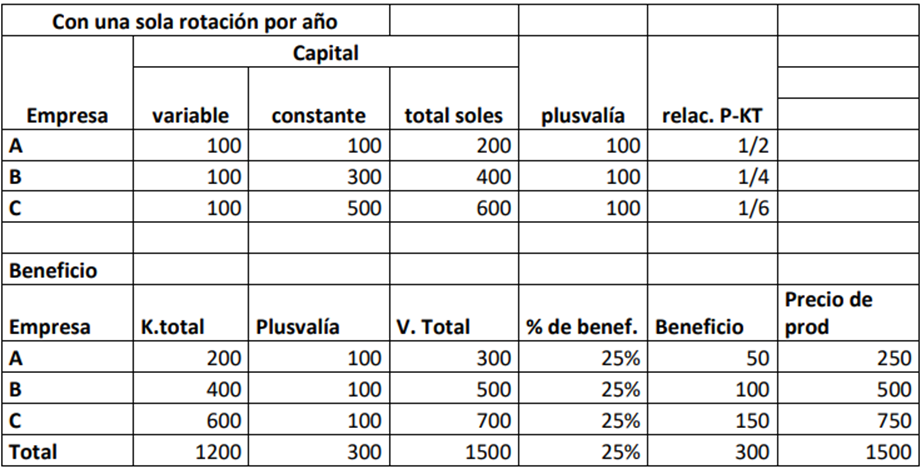
\includegraphics{Figura1.png}

}

\end{figure}

Vamos a ver cómo es lo que se genera la plusvalía y como se puede hacer
el cálculo inicial del beneficio

\begin{itemize}
\item
  Se va a realizar solo una rotación del capital
\item
  Se observa una empresa de A, B Y C que son empresas del mismo tipo
\item
  en la que el capital variable o sea el capital destinado al pago de
  remuneraciones o de salarios viene a ser iguales para todos 100.
\item
  sin embargo, se diferencian en la inversión que han hecho para el
  capital constante o sea maquinaria, equipo, muebles, inmuebles,
  materias primas e insumos.
\item
  El capital del total de soles es la suma del capital variable y el
  capital constante por ejemplo de la empresa A: 100+100=200.
\item
  Por la definición de la plusvalía: la plusvalía que genera la mano de
  obra es al 100\%. En conclusión, diremos que las tres empresas tienen
  el mismo nivel de plusvalía, dado que las tres empresas han invertido
  el mismo monto en el contrato del personal, pago de remuneraciones o
  de salarios a sus trabajadores, para homogeneizar con los textos
  diremos obreros. Ósea al 100\% prácticamente son iguales.
\item
  Si relacionamos con el capital total la plusvalía, sería que la
  empresa más pequeña que invierte 200, obtendría el 50\% de
  rentabilidad o sea el 1/2; el 50\% de su inversión obtendría la
  primera empresa con una menor inversión. La empresa B hizo una
  inversión de 400 pero solo obtiene una plusvalía del 25\% o sea solo
  la cuarta parte (1/4). Y la empresa más grande que invierte 600
  estaría obteniendo una plusvalía de la sexta parte (1/6) de su
  inversión.
\item
  Entonces vemos un caso en el que la empresa más pequeña gana más que
  la más grande, entonces no habría incentivo para invertir por lo que
  todos competirán para ser el más pequeño. Pero la realidad no es así,
  pero la tasa de la plusvalía es al 100\% todos tienen la misma
  plusvalía
\item
  Si nosotros queremos relacionar la cuota de la plusvalía, es la
  plusvalía sobre el capital variable sería 1 o sea el 100\%, el grado
  de explotación de estas empresas es al 100\%.
\item
  Sin embargo, nosotros debemos de buscar una media, no podemos trabajar
  con el trabajo socialmente necesario, la productividad, la intensidad.
  En la práctica no es el más pequeño el más eficiente pero tampoco se
  toma en consideración al más grande si no se considera la media, en
  este caso tomamos la tasa media de las empresas en cuanto a la
  relación de la plusvalía y el capital variable en este caso seria 1/4
  (25\%)
\item
  Ahora vamos a ver el concepto del beneficio: tenemos las tres
  empresas, pero ya el beneficio trabaja con el concepto del capital
  total; y tenemos 200, 400 y 600 y la plusvalía fue de 100, 100 y 100
  para las tres empresas, ahora sumamos al capital total la plusvalía
  tenemos el valor total 300, 500 y 700. La economía en su conjunto o
  sea el valor total de la producción generaría un valor total de 1500
  entonces hasta aquí tenemos la plusvalía. Ahora se tiene que trabajar
  el beneficio considerando la tasa media que es el 25\%, ahora si
  agarramos el 25\% del capital total: 25\% (200) =50, 25\% (400) =100 y
  el 25\% (600) =150. Entonces el precio del producto sería sumando el
  capital total y del beneficio o sea para la empresa A, B y C sería:
  200+50=250, 400+100=500 y 600+150=750 respectivamente.
\item
  En conclusión, sacamos que el total del valor total y el total del
  precio del producto son iguales de 1500 no ha variado, lo que ha
  pasado es que se ha reordenado la distribución de la riqueza, porque
  ahora si es correcto que el quien invierte menos gane menos y ahora si
  hay incentivo para que la empresa crezca porque aquí hay una inversión
  de 600 hay un premio. Y ahora ya hay una tasa de beneficio que ha
  ingresado a trabajar en relación con el capital, gracias a este
  comportamiento es que las empresas tienen incentivos para invertir.
  Finalmente, el que está funcionando en el mercado es la búsqueda del
  beneficio no de la plusvalía, pero a mayor capital invertido vamos a
  obtener una mayor tasa de beneficio que está cubierto por el capital.
\item
  En la parte superior del cuadro lo que hemos visto es que si solo
  consideramos el capital variable tendríamos una plusvalía la cuota de
  plusvalía en relación con la remuneración, pero esta se reduce si se
  quiere tanto y cuanto las empresas compiten en el mercado buscando
  beneficios. Entonces la empresa más grande que tiene maquinaria y
  equipo más moderno será él quien obtenga una tasa de beneficio más
  alto al interior está la plusvalía, el único que genera la riqueza es
  la fuerza de trabajo. La maquinaria y equipos, la materia prima e
  insumos, etc. Solo transfiere valor.
\end{itemize}

\begin{quote}
Si nosotros hablamos de la plusvalía vamos a hablar de capital constante
y capital variable (si solo tomamos solo el capital variable (la mano de
obra) nos sale la plusvalía) y si tomamos con el capital total la
relación de la plusvalía lo que estamos haciendo es pasarlo a un
concepto de beneficio\ldots ojo es como un resumen
\end{quote}

\begin{itemize}
\tightlist
\item
  Si hablamos de beneficio: hablamos del capital circulante y del
  capital fijo y ahí desaparece el concepto de plusvalía porque ya no
  estamos relacionándolo solo con el monto invertido de remuneraciones y
  salarios o vale decir del capital variable.
\end{itemize}

\hypertarget{renta-diferencial}{%
\section{Renta diferencial}\label{renta-diferencial}}

Es como una definición usual como lo llaman muchos en el capitalismo de
la ganancia aquí en este caso tenemos que ver el manejo de los
beneficios en la actividad agropecuaria no en la fábrica o en las
empresas que se desarrollan en la ciudad si no en el área rural.
Entonces una de las fuentes que surge de hecho en el capitalismo es el
beneficio que debe lograr el capitalista o el empresario luego de tener
beneficios normales o puede obtener beneficios extraordinarios o un
super beneficio entre los diversos tipos de beneficios, lo que aquí
interesa lo relacionado con el campo de la producción en relación con
los medios de producción particularmente aplicado en el área rural o sea
en el campo agropecuario. En el campo industrial como ya sabemos de qué
las empresas que incorporan maquinaria y equipo de última generación en
el corto plazo van a obtener beneficios extraordinarios, entonces eso es
lo que les empuja a hacer cambios o mejoras permanentes en la tecnología
como las fábricas que van a estar en una lucha feroz de incorporar
mejoras tecnológicas. Al tratar de obtener beneficios extraordinarios se
le llama como renta diferencial, en este caso nos interesa la parte en
la que la producción que gracias a los medios de producción especiales o
particulares, o ventajas especiales que tiene los tipos de terrenos o
ubicación, etc. Produce a un precio de costos menores, y se imponen
condiciones de producción dominantes. Aquí el que se va a imponer en el
mercado es el precio del peor terreno en el agro, en la industria el que
se impone en el mercado es el que produce a los costos más bajos
posibles, y cada vez la tendencia de los costos es a la baja para
emplear los beneficios y eso hace que quiebren las empresas.

En el sector agropecuario tiene condiciones especiales la parte de la
producción cuando gracias a los medios de producción especiales o
particulares que le permiten obtener ventajas y producen a un precio de
costos inferiores el que se va a imponer en el mercado son las
condiciones de producción dominante. Entonces el que se impone es el
precio del peor terreno: por ejemplo, el papero llega al mercado y
piensa en vender a 1 sol y resulta que encuentra que la papa está a 1.20
en el mercado, por lo que va a vender a 1.20 o sea se está adecuando al
precio que encontró en el mercado, en este caso es el precio que está
imponiéndose el peor terreno del pequeño productor agricultor con los
costos que ha alcanzado esa empresa pero todavía le permite estar en el
mercado, es donde qué ocurre este razonamiento los productos importados
destruyen al agricultor o sea al pequeño agricultor por el mismo hecho
de que pueden vender a 1.00 y quieres vender a 1.20 entonces te adecuas
al precio del producto importado lo cual cae a la pérdida. Entonces
tenemos una renta diferencial bajo condiciones especiales.

\textbf{Renta diferencial por distinta fertilidad}

Los tipos de terreno que nosotros tenemos que nos brinda la naturaleza,
no tienen la misma fertilidad, los diferentes tipos de terreno presentan
o son más fértiles que otros, unos son más pedregosos otros con tierra
negra, otros son con pura arena.

Asumamos que la inversión es la misma en los diferentes tipos de
terrenos, unos más fértiles que otros. La inversión por parte de los
capitalistas o de los productores es la misma, la diferencia que vamos a
encontrar de este beneficio extraordinario o super beneficio se debe
principal, fundamental y únicamente por las leyes especiales de la renta
diferencial. En este caso se encuentran comprometidos todos los
recursos, todas las fuerzas productivas incluido por ejemplo las aguas.

El super beneficio se origina por la desigual productividad de los
diversos tipos de terreno y que se convierten en permanentes: por
ejemplo, el terreno es pedregoso los rendimientos van a ser menores, la
productividad de la mano de obra va a ser menor por que el nivel de
inversión en la que estamos partiendo es el mismo en los tipos de
terreno de parte de los agricultores.

En la agricultura no son los costos de producción los que determinan el
precio de costo o costos de factores, pero en la industria sí, hay
agricultores aun cuando el precio del producto que venden no les permite
recuperar toda su inversión están en el mercado transitoriamente en esa
cosecha que después se le pueden retirar. Dado que el terreno peor será
explotado solos y la insuficiencia de la oferta ha hecho aumentar los
precios a tal punto que el cultivo del peor terreno sea rentable y el
que se impone en el mercado son los costos de producción necesarios del
peor terreno. Entonces cuando la oferta es relativamente menor y la
demanda sube los precios lo suficiente como para ser rentable a la
actividad agropecuaria en el peor terreno y siempre habrá peores
terrenos, pero esos son los que se imponen en el mercado. Por ejemplo,
en el Perú cuando el petróleo está 10 soles el galón no hay incentivos
para buscar pozos petroleros en el mundo menos en el Perú nos conviene
importarlos, pero si el precio del petróleo a nivel mundial pasa los 120
dólares que paso en el 2008 que llegó a 150 dólares en ese momento ya se
hace rentable producir o buscar como en el Perú dado los volúmenes que
explotamos ya que hay incentivos, igual en agro habrá un precio al cual
será rentable o habrá incentivo para ingresar a explotar dentro de los
peores terrenos entonces si había un terreno que siempre ha estado
descansando e ingresan o comienzan a sembrar y que los precios del
cultivo justifican la puesta en producción en ese tipo de terreno y el
costo de producción de ese terreno va reflejar el precio a costo de
factores en el mercado y a este precio se van a adecuar los otros.

La población aumenta ahí donde se desarrolla la industria y no es donde
que se desarrolla la actividad agropecuaria, la concentración de la
población se dan en las zonas dónde están las fábricas o las actividades
propias de la zona urbana y ahí donde nos concentramos. y con ello
aumenta la demanda de medios de subsistencia. Por lo que es necesario
cultivar más y nuevas tierras o mejoras tecnológicas, porque también es
cierto de que los rendimientos y la productividad a la par del aumento
de la población o incluso a mayor velocidad del crecimiento de la
población ha aumentado los rendimientos y la productividad. Con este
caso Malthus tendría la razón ya hubiera desaparecido ya que decía
geométricamente crece la población y aritméticamente los alimentos, nos
es así en la actualidad lo que hay más son los alimentos. Por ejemplo,
antes por una hectárea de tierra se sacaba dos toneladas en el mejor de
los casos 2.5 toneladas métricas de papa ahora sacan 40 toneladas de
papa por hectárea para ser rentable, entonces los rendimientos son
altísimos y la productividad ha aumentado. Hay que tener claro de que el
que se impone a costo de factores en el mercado es el costo de
producción o el precio que es el costo del peor terreno que ha entrado
en producción gracias a los precios que se han incrementado como
resultado de la insuficiencia de la oferta, dicho de otro modo, cuando
la oferta es menor que la demanda.

\textbf{Renta diferencial por distinta fertilidad} (tenemos diferentes
tipos de terreno con diferentes niveles de fertilidad son propias de la
naturaleza)

\begin{longtable}[]{@{}
  >{\raggedright\arraybackslash}p{(\columnwidth - 16\tabcolsep) * \real{0.1218}}
  >{\raggedright\arraybackslash}p{(\columnwidth - 16\tabcolsep) * \real{0.0897}}
  >{\raggedright\arraybackslash}p{(\columnwidth - 16\tabcolsep) * \real{0.1410}}
  >{\raggedright\arraybackslash}p{(\columnwidth - 16\tabcolsep) * \real{0.1282}}
  >{\raggedright\arraybackslash}p{(\columnwidth - 16\tabcolsep) * \real{0.0577}}
  >{\raggedright\arraybackslash}p{(\columnwidth - 16\tabcolsep) * \real{0.1026}}
  >{\raggedright\arraybackslash}p{(\columnwidth - 16\tabcolsep) * \real{0.1154}}
  >{\raggedright\arraybackslash}p{(\columnwidth - 16\tabcolsep) * \real{0.1090}}
  >{\raggedright\arraybackslash}p{(\columnwidth - 16\tabcolsep) * \real{0.1346}}@{}}
\toprule\noalign{}
\begin{minipage}[b]{\linewidth}\raggedright
\textbf{Tipo de terreno}
\end{minipage} & \begin{minipage}[b]{\linewidth}\raggedright
\textbf{Producción}
\end{minipage} & \begin{minipage}[b]{\linewidth}\raggedright
\textbf{Capital anticipado}
\end{minipage} & \begin{minipage}[b]{\linewidth}\raggedright
\textbf{Tasa de ganancia}
\end{minipage} & \begin{minipage}[b]{\linewidth}\raggedright
\textbf{Total}
\end{minipage} & \begin{minipage}[b]{\linewidth}\raggedright
\textbf{Precio de TM}
\end{minipage} & \begin{minipage}[b]{\linewidth}\raggedright
\textbf{Total de venta}
\end{minipage} & \begin{minipage}[b]{\linewidth}\raggedright
\textbf{Precio por TM}
\end{minipage} & \begin{minipage}[b]{\linewidth}\raggedright
\textbf{Renta territorial}
\end{minipage} \\
\midrule\noalign{}
\endhead
\bottomrule\noalign{}
\endlastfoot
A & 450 & 3200 & 25\% & 4000 & 8.89 & 4500 & 10 & 500 \\
B & 400 & 3200 & 25\% & 4000 & 10 & 4000 & 10 & 0 \\
\end{longtable}

\begin{itemize}
\item
  Tenemos dos empresas con dos tipos de terreno: tipo A y tipo B, lo que
  nos interesa es el rendimiento. En este caso el terreno tipo A se
  obtiene 450 y en el tipo B obtenemos 400.
\item
  El capital que se ha destinado para producir en estos tipos de terreno
  hemos puesto en los dos casos 3200 soles
\item
  La tasa de ganancia se obtiene del porcentaje del beneficio el 25\%
  del cuadro del beneficio
\item
  El valor total sale con el 25\% del capital anticipado: 25\        (3200)
  =800→3200+800=400 y de terreno B es: 25\% (3200) =800→3200+800=4000.
\item
  Lo que quiere decir el precio por tonelada métrica vendría a ser en el
  caso del terreno tipo A el 8.89 y en el segundo caso sería 10: se
  obtuvo 4000/450=8.89 y 4000/400=10.
\item
  El precio que se impone en el mercado es 10, el precio más alto es el
  que se impone en el mercado mientras en la industria es al revés ya
  que el precio más bajo es el que se impone en el mercado la tendencia
  es eliminar. En este caso el que se impone en el mercado es el más
  alto y es 10 y el terreno de tipo A se adecua al precio más alto.
\item
  El total de venta será con el nuevo precio para el tipo de terreno A
  de 450\_10=4500 y del tipo de terreno B: 400\_10=4000.
\item
  La renta diferencial por efecto de fertilidad del terreno va a ser de
  500 para el productor del terreno A, este es un beneficio
  extraordinario no significa que el productor de la B no esté ganando,
  si no si está ganando tiene una tasa de beneficio del 25\%. Pero por
  encima del beneficio el productor del tipo de terreno A está
  obteniendo un beneficio extraordinario o un super beneficio por encima
  de todo
\end{itemize}

\begin{longtable}[]{@{}
  >{\raggedright\arraybackslash}p{(\columnwidth - 16\tabcolsep) * \real{0.1218}}
  >{\raggedright\arraybackslash}p{(\columnwidth - 16\tabcolsep) * \real{0.0897}}
  >{\raggedright\arraybackslash}p{(\columnwidth - 16\tabcolsep) * \real{0.1410}}
  >{\raggedright\arraybackslash}p{(\columnwidth - 16\tabcolsep) * \real{0.1282}}
  >{\raggedright\arraybackslash}p{(\columnwidth - 16\tabcolsep) * \real{0.0577}}
  >{\raggedright\arraybackslash}p{(\columnwidth - 16\tabcolsep) * \real{0.1026}}
  >{\raggedright\arraybackslash}p{(\columnwidth - 16\tabcolsep) * \real{0.1154}}
  >{\raggedright\arraybackslash}p{(\columnwidth - 16\tabcolsep) * \real{0.1090}}
  >{\raggedright\arraybackslash}p{(\columnwidth - 16\tabcolsep) * \real{0.1346}}@{}}
\toprule\noalign{}
\begin{minipage}[b]{\linewidth}\raggedright
\textbf{Tipo de terreno}
\end{minipage} & \begin{minipage}[b]{\linewidth}\raggedright
\textbf{Producción}
\end{minipage} & \begin{minipage}[b]{\linewidth}\raggedright
\textbf{Capital anticipado}
\end{minipage} & \begin{minipage}[b]{\linewidth}\raggedright
\textbf{Tasa de ganancia}
\end{minipage} & \begin{minipage}[b]{\linewidth}\raggedright
\textbf{Total}
\end{minipage} & \begin{minipage}[b]{\linewidth}\raggedright
\textbf{Precio de TM}
\end{minipage} & \begin{minipage}[b]{\linewidth}\raggedright
\textbf{Total de venta}
\end{minipage} & \begin{minipage}[b]{\linewidth}\raggedright
\textbf{Precio por TM}
\end{minipage} & \begin{minipage}[b]{\linewidth}\raggedright
\textbf{Renta territorial}
\end{minipage} \\
\midrule\noalign{}
\endhead
\bottomrule\noalign{}
\endlastfoot
A & 450 & 3200 & 25\% & 4000 & 8.89 & 5625 & 12.5 & 1625 \\
B & 400 & 3200 & 25\% & 4000 & 10 & 5000 & 12.5 & 1000 \\
C & 320 & 3200 & 25\% & 4000 & 12.5 & 4000 & 12.5 & 0 \\
\end{longtable}

\begin{itemize}
\item
  En este caso entra en producción un peor terreno con menor fertilidad,
  subieron los precios y se hace rentable y se justifica ingresar a este
  terreno, este terreno A y B siguen produciendo lo mismo 450 y 400, en
  tipo de terreno tiene un volumen de producción de 320 esta es la
  cosecha.
\item
  El capital invertido sigue siendo el mismo.
\item
  La tasa de ganancia sigue el mismo del 25\%
\item
  El valor total se calcula de la misma forma del primer cuadro
\item
  Los precios del tipo de terreno de A y B es el mismo resultado que del
  primer cuadro, pero para el tipo de terreno C será 4000/320=12.5
\item
  El precio que se impone en el mercado es de 12.5, cómo ha ingresado un
  peor terreno a la producción de la actividad agropecuaria, ahora el
  ingreso total de cada uno de ellos va a aumentar en el caso de A y B,
  a comparación del primer caso la B que no tenía una renta diferencial
  o el super ahora va obtener 1000 de beneficio extraordinario. Y en el
  caso del terreno A va a aumentar mucho más a 1625 de beneficio
  extraordinario antes tenía solo de 500 gracias a que ha ingresado al
  mercado de tipo C ahora obtiene una renta diferencial más alta y el
  tipo B ha obtenido una renta diferencial.
\end{itemize}

\begin{longtable}[]{@{}
  >{\raggedright\arraybackslash}p{(\columnwidth - 16\tabcolsep) * \real{0.1218}}
  >{\raggedright\arraybackslash}p{(\columnwidth - 16\tabcolsep) * \real{0.0897}}
  >{\raggedright\arraybackslash}p{(\columnwidth - 16\tabcolsep) * \real{0.1410}}
  >{\raggedright\arraybackslash}p{(\columnwidth - 16\tabcolsep) * \real{0.1282}}
  >{\raggedright\arraybackslash}p{(\columnwidth - 16\tabcolsep) * \real{0.0577}}
  >{\raggedright\arraybackslash}p{(\columnwidth - 16\tabcolsep) * \real{0.1026}}
  >{\raggedright\arraybackslash}p{(\columnwidth - 16\tabcolsep) * \real{0.1154}}
  >{\raggedright\arraybackslash}p{(\columnwidth - 16\tabcolsep) * \real{0.1090}}
  >{\raggedright\arraybackslash}p{(\columnwidth - 16\tabcolsep) * \real{0.1346}}@{}}
\toprule\noalign{}
\begin{minipage}[b]{\linewidth}\raggedright
\textbf{Tipo de terreno}
\end{minipage} & \begin{minipage}[b]{\linewidth}\raggedright
\textbf{Producción}
\end{minipage} & \begin{minipage}[b]{\linewidth}\raggedright
\textbf{Capital anticipado}
\end{minipage} & \begin{minipage}[b]{\linewidth}\raggedright
\textbf{Tasa de ganancia}
\end{minipage} & \begin{minipage}[b]{\linewidth}\raggedright
\textbf{Total}
\end{minipage} & \begin{minipage}[b]{\linewidth}\raggedright
\textbf{Precio de TM}
\end{minipage} & \begin{minipage}[b]{\linewidth}\raggedright
\textbf{Total de venta}
\end{minipage} & \begin{minipage}[b]{\linewidth}\raggedright
\textbf{Precio por TM}
\end{minipage} & \begin{minipage}[b]{\linewidth}\raggedright
\textbf{Renta territorial}
\end{minipage} \\
\midrule\noalign{}
\endhead
\bottomrule\noalign{}
\endlastfoot
X & 500 & 3200 & 25\% & 4000 & 8.00 & 5000 & 12.5 & 1000 \\
A & 450 & 3200 & 25\% & 4000 & 8.89 & 4500 & 12.5 & 500 \\
B & 400 & 3200 & 25\% & 4000 & 10 & 4000 & 12.5 & 0 \\
\end{longtable}

\begin{itemize}
\tightlist
\item
  Este tercer caso es que ahora ha ingresado un mejor terreno (podría
  haber estado en descanso) o sea mejor que el A y B, La B va a seguir
  siendo el peor terreno, este mejor al tener mayor fertilidad va tener
  una mayor renta diferencial y no afecta a la renta diferencial del
  terreno del A, porque sigue manteniendo el precio a costo de factores
  del terreno del tipo B que se vio en el primer caso.
\end{itemize}

\textbf{Renta diferencial por distancia del mercado}

\begin{longtable}[]{@{}
  >{\centering\arraybackslash}p{(\columnwidth - 12\tabcolsep) * \real{0.0457}}
  >{\centering\arraybackslash}p{(\columnwidth - 12\tabcolsep) * \real{0.1600}}
  >{\centering\arraybackslash}p{(\columnwidth - 12\tabcolsep) * \real{0.1200}}
  >{\centering\arraybackslash}p{(\columnwidth - 12\tabcolsep) * \real{0.1886}}
  >{\centering\arraybackslash}p{(\columnwidth - 12\tabcolsep) * \real{0.1314}}
  >{\centering\arraybackslash}p{(\columnwidth - 12\tabcolsep) * \real{0.1200}}
  >{\centering\arraybackslash}p{(\columnwidth - 12\tabcolsep) * \real{0.2343}}@{}}
\toprule\noalign{}
\begin{minipage}[b]{\linewidth}\centering
\textbf{Lote}
\end{minipage} & \begin{minipage}[b]{\linewidth}\centering
\textbf{Distancia del mercado KM}
\end{minipage} & \begin{minipage}[b]{\linewidth}\centering
\textbf{Producción en T.M}
\end{minipage} & \begin{minipage}[b]{\linewidth}\centering
\textbf{Precio del producto en chacra}
\end{minipage} & \begin{minipage}[b]{\linewidth}\centering
\textbf{Costo de transporte}
\end{minipage} & \begin{minipage}[b]{\linewidth}\centering
\textbf{Precio de mercado}
\end{minipage} & \begin{minipage}[b]{\linewidth}\centering
\textbf{Renta territorial (Renta diferencial)}
\end{minipage} \\
\midrule\noalign{}
\endhead
\bottomrule\noalign{}
\endlastfoot
A & 5 & 400 & 4000 & 20 & 4400 & 380 \\
B & 50 & 400 & 4000 & 200 & 4400 & 200 \\
C & 100 & 400 & 4000 & 400 & 4400 & 0 \\
\end{longtable}

\begin{itemize}
\item
  La renta diferencial se presenta por distancia al mercado, tenemos
  terrenos no cercanos a la ciudad, pero los que están más cerca de la
  ciudad tienen ventajas
\item
  En fertilidad son iguales, el ceteris paribus también son iguales lo
  que se diferencian es en la distancia al mercado.
\item
  En este caso tenemos 3 tipos de terreno el A a 5 km al mercado, el
  otro a 50 km y el otro a 100 km
\item
  El volumen de producción es igual, todos producen igual y han
  invertido igual
\item
  El precio del producto en chacra es de 4000 en este ya está incluido
  el beneficio.
\item
  El costo de transporte aquí está la diferencia que es según la
  distancia en este caso es de 20, 200 y de 400, se deduce que el precio
  del transporte por kilómetro es de 4
\item
  Al mercado se llega con el precio del producto en el mercado se toma
  el terreno más lejano del mercado es por eso por lo que se entra es
  con 4400, el más lejano es el que se impone en el mercado y esta gana
  solo el beneficio más no el beneficio extraordinario o la renta
  diferencial de la distancia del mercado.
\item
  Un ejemplo es la cebolla de Ayacucho entra con el precio de Arequipa.
\item
  Por eso es importante mejorar la infraestructura vial para reducir los
  costos de transporte y el tiempo.
\end{itemize}

\textbf{Mejorando la calidad de la tierra, mayor empleo de trabajo,
mayor inversión de k, sea en salarios, abonos, instrumentos, etc.}

\begin{itemize}
\item
  Mejorando la calidad de la tierra: siempre los campesinos o los
  pequeños agricultores no son capaces de mejorar su tipo de terreno o
  sea no son capaces de sacar piedras, rastrillar, hacer limpieza, entre
  otros, trabajan sobre lo mismo
\item
  Se puede introducir mejor mano de obra, o sea se puede hacer más
  intensivo en mano de obra, por ejemplo, de repente se está usando muy
  poca mano de obra, debemos hacer más intenso el uso del trabajo.
\item
  Puedes adaptar la maquinaria a la necesidad de tu terreno
\item
  Las inversiones pueden ser en bienes de capital como en: salarios, de
  repente se puede obtener mano de obra calificada a un precio
  relativamente al alcance de tu centro de explotación agropecuaria. Si
  se tiene 25 a 30 hectáreas a mes podrías tener una visita de un
  ingeniero especialista en esa área como para que supervise y reconozca
  los problemas, pero esto no quiere decir que tú vas a dejar de
  practicar tu experiencia propia, porque tal vez el profesional de alto
  nivel tiene un punto de vista y de repente no se adapta a tu realidad.
  Ahora veremos el uso de los abonos, tendríamos que ver qué hacen los
  químicos, biólogos, los agrónomos, y saber que combinaciones realizan,
  por ejemplo, si hemos sembrado papa que productos podemos sembrar para
  la siguiente para rotar y en qué abonos debemos invertir. En
  maquinarias y equipos (instrumentos), instrumentos más modernos o
  nuevos, por ejemplo, de paltos siguen podando con motosierra, pero con
  el instrumento más moderno sería con la motosierra de altura y no
  pierdes el tiempo.
\end{itemize}

\begin{longtable}[]{@{}
  >{\raggedright\arraybackslash}p{(\columnwidth - 14\tabcolsep) * \real{0.0588}}
  >{\raggedright\arraybackslash}p{(\columnwidth - 14\tabcolsep) * \real{0.0980}}
  >{\raggedright\arraybackslash}p{(\columnwidth - 14\tabcolsep) * \real{0.0392}}
  >{\raggedright\arraybackslash}p{(\columnwidth - 14\tabcolsep) * \real{0.1569}}
  >{\raggedright\arraybackslash}p{(\columnwidth - 14\tabcolsep) * \real{0.1961}}
  >{\raggedright\arraybackslash}p{(\columnwidth - 14\tabcolsep) * \real{0.1176}}
  >{\raggedright\arraybackslash}p{(\columnwidth - 14\tabcolsep) * \real{0.1667}}
  >{\raggedright\arraybackslash}p{(\columnwidth - 14\tabcolsep) * \real{0.1667}}@{}}
\toprule\noalign{}
\begin{minipage}[b]{\linewidth}\raggedright
L de K
\end{minipage} & \begin{minipage}[b]{\linewidth}\raggedright
Producción
\end{minipage} & \begin{minipage}[b]{\linewidth}\raggedright
K
\end{minipage} & \begin{minipage}[b]{\linewidth}\raggedright
Tasa de ganancia
\end{minipage} & \begin{minipage}[b]{\linewidth}\raggedright
Costos de producción
\end{minipage} & \begin{minipage}[b]{\linewidth}\raggedright
Precio X T.M
\end{minipage} & \begin{minipage}[b]{\linewidth}\raggedright
Precio de mercado
\end{minipage} & \begin{minipage}[b]{\linewidth}\raggedright
Renta territorial
\end{minipage} \\
\midrule\noalign{}
\endhead
\bottomrule\noalign{}
\endlastfoot
A1 & 450 & 3200 & 25\% & 4000 & 10 & 4500 & 500 \\
A2 & 420 & 3200 & 25\% & 4000 & 10 & 4200 & 200 \\
Total & 870 & 6400 & 25\% & 8000 & 10 & 8700 & 700 \\
B & 400 & 3200 & 25\% & 4000 & 10 & 4000 & 0 \\
\end{longtable}

\begin{itemize}
\item
  Como ya hemos visto la inversión de capital que se necesita visto que
  hay que hacer diversas inversiones adicionales en el terreno en el
  cual hemos incorporado la actividad agropecuaria.
\item
  En este caso tenemos terreno A1 y B, en el A1 vamos a hacer mejoras,
  por ejemplo, el tipo de terreno podemos mejorar, podemos hacer
  inversiones adicionales, de cambios sustanciales en la explotación del
  terreno A.
\item
  En el A1 y B tenemos un volumen de producción de 450 y de 400, tenemos
  el precio a costos de factores y el precio que se impone es de 10.
\item
  Como resultado de las mejoras en la explotación A en el terreno A2
  vamos a obtener un rendimiento más alto que el B de 420. Si bien es
  cierto al inicio ya teníamos una renta diferencial o renta territorial
  de 500 y la B no tenía renta extraordinaria. Ahora por las mejoras que
  hemos introducido un lote adicional de A2 de la explotación agraria A,
  vamos a obtener una renta diferencial de 200, esto es el incentivo en
  el sector agropecuario para mejorar la calidad de la tierra o del
  terreno para hacer mayor empleo del trabajo, mayor inversión de
  capital que puede ser en los salarios, en abonos, e insecticidas,
  pesticidas, maquinarias y equipo, entre otros. Dependiendo de las
  necesidades por ejemplo de instalación de agua puedes mejorar,
  represas artesanales y estos generan más rendimiento.
\item
  La explicación está en mayor inversión y la mejora que se efectúa en
  la explotación.
\end{itemize}

En la clase anterior vimos la: renta diferencial por diferencia en la
fertilidad, por la distancia al mercado osea, la cercanía que se tiene a
las zonas de distribución generan un beneficio extraordinario, también
vimos cómo podíamos mejorar la calidad y obtener beneficios
extraordinarios o haciendo que haya mayor inversión, a través de un
incentivo para la inversión salarios también o sea podemos tener
salarios bajos, incorporación de maquinaria y equipo, abonos nuevos o
mejor uso de las mismas, la mayor intensidad de trabajo en la
explotación, también podemos obtener renta por rotación pero entremos a
ver la renta absoluta.

\textbf{Renta diferencial.} El capitalista puede obtener unos beneficios
extraordinarios gracias a las ventajas produce a un precio inferior. Con
la misma inversión producirá más volúmenes. Donde se concentra la
población el precio de los terrenos aumenta.

\textbf{Renta absoluta.}

Transferir al precio de mercado, generando renta diferencial.

El monopolio del terrateniente sin el permiso de ello no hay explotación
posible.

el peor terreno se rotaron siempre y cuando los precios hayan subido lo
suficiente para estar por encima de los precios de producción. De modo
que le aseguré a él también una súper ganancia.

La renta absoluta aparte de lo que hemos visto de la renta diferencial o
la renta territorial, si se quiere refiere al hecho del monopolio del
propietario, del terrateniente, el permiso de él, no hay explotación si
los dueños del terreno que están en descanso que no se dedican al sector
agrario y que si ellos no aceptan entre en producción, simplemente no
puede, no se explota esas tierras, entonces tenemos tierras en descanso
en buenas condiciones en este caso, como decíamos el peor terreno, se o
entrar en producción siempre y cuando los precios hayan subido lo
suficiente como para estar por encima de los precios o de los precios de
los costos de producción por encima de los precios de producción o a
precios a costo de factores de modo que este precio.

Producción con una sola rotación por año

\begin{longtable}[]{@{}
  >{\raggedright\arraybackslash}p{(\columnwidth - 10\tabcolsep) * \real{0.1111}}
  >{\raggedright\arraybackslash}p{(\columnwidth - 10\tabcolsep) * \real{0.2020}}
  >{\raggedright\arraybackslash}p{(\columnwidth - 10\tabcolsep) * \real{0.2121}}
  >{\raggedright\arraybackslash}p{(\columnwidth - 10\tabcolsep) * \real{0.1717}}
  >{\raggedright\arraybackslash}p{(\columnwidth - 10\tabcolsep) * \real{0.1313}}
  >{\raggedright\arraybackslash}p{(\columnwidth - 10\tabcolsep) * \real{0.1717}}@{}}
\toprule\noalign{}
\begin{minipage}[b]{\linewidth}\raggedright
\textbf{Empresa}
\end{minipage} & \begin{minipage}[b]{\linewidth}\raggedright
\textbf{Capital Variable}
\end{minipage} & \begin{minipage}[b]{\linewidth}\raggedright
\textbf{Capital Constante}
\end{minipage} & \begin{minipage}[b]{\linewidth}\raggedright
\textbf{Total (soles)}
\end{minipage} & \begin{minipage}[b]{\linewidth}\raggedright
\textbf{Plusvalía}
\end{minipage} & \begin{minipage}[b]{\linewidth}\raggedright
\textbf{Relación P-KT}
\end{minipage} \\
\midrule\noalign{}
\endhead
\bottomrule\noalign{}
\endlastfoot
A & 100 & 100 & 200 & 100 & 1/2 \\
B & 300 & 100 & 400 & 100 & 1/4 \\
C & 500 & 100 & 600 & 100 & 1/6 \\
\end{longtable}

También se presentaría renta diferencial si hacemos varias rotaciones
osea, sacamos dos cosechas se duplica la renta diferencial, si sacamos
tres cosechas se triplica, las hortalizas se puede sacar 4 cosechas,
entonces entra el juego de tiempo de producción y lógicamente la
rotación técnica que se pueda dar en la lechuga, espinaca, coliflor,
espinaca, estos produce salir hasta 4.

En este caso vemos la relación de la plusvalía con en relación a la
inversión total, que viene a ser mucho menos que si la relacionamos sólo
con el capital variable.

La renta absoluta se presenta porque va a ingresar las tierras que están
en descanso como resultado de la propiedad privada, tú puedes tener tu
terreno x no entras en cultivo, mientras tú ves que es muy sacrificado,
entonces va a llegar un momento en que tu como agricultor vas a ir donde
el dueño de esas tierras y va decir alquilame.

además de cubrir el alquiler, el precio de tu producto de origen
agropecuario estén suficientemente altos como para cubrir esos alquiler,
además el agricultor aparte del beneficio normal, de la renta
diferencial, le permita obtener otra renta, otro ingreso adicional por
cultivo que viene a ser la renta absoluta.

Por rotación

\begin{longtable}[]{@{}
  >{\centering\arraybackslash}p{(\columnwidth - 6\tabcolsep) * \real{0.1833}}
  >{\centering\arraybackslash}p{(\columnwidth - 6\tabcolsep) * \real{0.2000}}
  >{\centering\arraybackslash}p{(\columnwidth - 6\tabcolsep) * \real{0.2167}}
  >{\centering\arraybackslash}p{(\columnwidth - 6\tabcolsep) * \real{0.4000}}@{}}
\toprule\noalign{}
\begin{minipage}[b]{\linewidth}\centering
\textbf{Empresa}
\end{minipage} & \begin{minipage}[b]{\linewidth}\centering
\textbf{Total, K}
\end{minipage} & \begin{minipage}[b]{\linewidth}\centering
\textbf{Plusvalía}
\end{minipage} & \begin{minipage}[b]{\linewidth}\centering
\textbf{Relación Plusvalía K}
\end{minipage} \\
\midrule\noalign{}
\endhead
\bottomrule\noalign{}
\endlastfoot
A & 200 & 100 & 0.5 \\
B & 200 & 100 & 0.5 \\
C & 150 & 100 & 0.67 \\
\end{longtable}

\begin{longtable}[]{@{}
  >{\raggedright\arraybackslash}p{(\columnwidth - 14\tabcolsep) * \real{0.1387}}
  >{\raggedright\arraybackslash}p{(\columnwidth - 14\tabcolsep) * \real{0.0876}}
  >{\raggedright\arraybackslash}p{(\columnwidth - 14\tabcolsep) * \real{0.0949}}
  >{\raggedright\arraybackslash}p{(\columnwidth - 14\tabcolsep) * \real{0.1314}}
  >{\raggedright\arraybackslash}p{(\columnwidth - 14\tabcolsep) * \real{0.1533}}
  >{\raggedright\arraybackslash}p{(\columnwidth - 14\tabcolsep) * \real{0.1533}}
  >{\raggedright\arraybackslash}p{(\columnwidth - 14\tabcolsep) * \real{0.1314}}
  >{\raggedright\arraybackslash}p{(\columnwidth - 14\tabcolsep) * \real{0.1095}}@{}}
\toprule\noalign{}
\begin{minipage}[b]{\linewidth}\raggedright
\textbf{Tipo de terreno}
\end{minipage} & \begin{minipage}[b]{\linewidth}\raggedright
\textbf{Producto}
\end{minipage} & \begin{minipage}[b]{\linewidth}\raggedright
\textbf{Precio TM}
\end{minipage} & \begin{minipage}[b]{\linewidth}\raggedright
\textbf{Precio General}
\end{minipage} & \begin{minipage}[b]{\linewidth}\raggedright
\textbf{Precio de Mercado}
\end{minipage} & \begin{minipage}[b]{\linewidth}\raggedright
\textbf{Renta Diferencial}
\end{minipage} & \begin{minipage}[b]{\linewidth}\raggedright
\textbf{Renta Absoluta}
\end{minipage} & \begin{minipage}[b]{\linewidth}\raggedright
\textbf{Renta Total}
\end{minipage} \\
\midrule\noalign{}
\endhead
\bottomrule\noalign{}
\endlastfoot
A & 450 & 8.88 & 12.5 & 15 & 1650 & 1125 & 27750 \\
B & 400 & 10 & 12.5 & 15 & 1000 & 1000 & 2000 \\
C & 320 & 12.5 & 12.5 & 15 & 0 & 800 & 800 \\
\end{longtable}

en este cuadro tenemos 3 terrenos, el producto es 450, 400 y 320, el
precio de cada uno a precio de costo de factores sería 8.88, 10 y 12.5.
El precio que se impone es el precio del peor terreno el 12.5. Entonces
con el precio 12.5 se obtiene la renta diferencial, la renta diferencial
es 1650 porque multiplicamos 8.88 por 450 y restamos la multiplicación
de 450 por 12.5. El último terreno no tiene renta diferencial, pero si
obtiene beneficio, no renuncia al beneficio. Ahora por la escasez de los
productos u otros factores ha aumentado a 15 soles por encima del precio
del peor terreno, la escasez de tierra ha hecho que ingresen tierras en
descanso. la diferencia de estos precios va general la renta absoluta,
en este caso 450\_15 -450\_12.5 da como resultado 1125, incluso el peor
terreno va a obtener una renta absoluta de 800 antes este terreno no era
partícipe de ello. Si sumamos las rentas sin considerar el beneficio
tendríamos 2775.

Entonces se puede ver que hay una renta adicional, la renta absoluta
cuando ingresan tierras en descanso en producción.

para que entren en producción tiene que haber subido los precios lo
suficiente para cubrir los alquileres y generar los beneficios aun
extraordinarios para el productor, sino estas tierras siguen
descansando. Estas tierras en descanso son resultados de la propiedad
privada, monopolio sobre las tierras.

El pequeño agricultor no produce con alta tecnología, sino ha estado
trabajando con insumos tradicionales, el efecto en el pequeño agricultor
va a ser mínimo, el efecto va ser en aquellos que van producir sus
producto con destino al extranjero, esos son los medianos y grandes,

\hypertarget{superioridad-tuxe9cnica-de-la-gran-explotaciuxf3n-1}{%
\section{Superioridad técnica de la gran
explotación}\label{superioridad-tuxe9cnica-de-la-gran-explotaciuxf3n-1}}

es hacer un comparativo de la explotación de la pequeña y la grande.

\begin{itemize}
\item
  Cuanto más diferente es la actividad agropecuaria, en más capitalista
  se convierte la actividad agropecuaria. si nosotros tenemos una
  agricultura bastante diferenciada entonces vamos a tener una
  agricultura orientada al mercado, esto nos da una idea de cómo es que
  la gran explotación va a comenzar a imponerse porque nuestro principal
  objetivo va ser abastecer al mercado en las mejores condiciones, para
  ello tenemos que diferenciarnos de otros productos. Mientras más se
  desarrolle una diferencia cualitativa desde el punto de vista de la
  tecnología entre la grande y pequeña explotación vamos a tener una
  agricultura capitalista.
\item
  En la antigüedad los medios de producción en el feudo no era más que
  lo del campesino,
\item
  El libre propietario produce con sus propios instrumentos, animales y
  obreros asalariados, entonces es cuando la pequeña explotación inicia
  a malgastar el tiempo de trabajo y los medios de trabajo
\item
  La diferencia primero se da en la casa y sus anexos
\item
  La diferencia entre la industria y la agricultura es que la
  agricultura aún es unidad con la economía doméstica.
\end{itemize}

Un comparativo

\begin{longtable}[]{@{}
  >{\raggedright\arraybackslash}p{(\columnwidth - 2\tabcolsep) * \real{0.4521}}
  >{\raggedright\arraybackslash}p{(\columnwidth - 2\tabcolsep) * \real{0.5479}}@{}}
\toprule\noalign{}
\begin{minipage}[b]{\linewidth}\raggedright
\textbf{01 gran explotación (20 ha)}
\end{minipage} & \begin{minipage}[b]{\linewidth}\raggedright
\textbf{50 pequeñas explotaciones (media ha)}
\end{minipage} \\
\midrule\noalign{}
\endhead
\bottomrule\noalign{}
\endlastfoot
01 cocina, 05 cocineros, 05 focos & 50 cocinas 50 cocineros 50 focos \\
01 establo con 100 reses & 50 establos \\
01 pozo de agua & 50 pozos \\
10 herramientas & 100 herramientas \\
\end{longtable}

Tenemos dos propiedades una grande y una pequeña, una explotación de 20
ha. en la gran explotación tiene todas sus comodidades, mientras en
pequeña explotación cada casa tiene un foco en suma 50 focos, ¿dónde hay
más costos? son pequeñas, y hay más costo.

Los linderos reducen el tamaño de las propiedades, lo hacen más
pequeños, y a raíz de estos cercos y la tecnología que no ha avanzado
también se reduce, Cuanto más pequeñas las propiedades más Linderos.
terreno perdido por cerco si el uso del arado entonces, Cuanto más
pequeña la explotación en mayores costos incurre.

En pequeña explotación hay mayor inversión de capital y sin embargo los
rendimientos y la productividad son menores, además el pequeño
agricultor es el menos capacitado y tiene menos acceso conocimiento, y
por lo tanto menos acceso de a la incorporación de tecnología de última
generación.

es importante en agrandar la propiedad, capacitar, ya no en la
producción porque ellos saben, sino capacitar en manejo de costos, en
mercados, como debe llegar y en qué momento

\hypertarget{rentabilidad-en-la-agricultura-1}{%
\section{Rentabilidad en la
Agricultura}\label{rentabilidad-en-la-agricultura-1}}

Lo vemos considerando incorporar subsidios para el agro solo así se va a
ser rentable.

Debe haber más profesionalismo, mayor incorporación, la agricultura en
la América Latina está sometida en una contradicción, porque por un lado
hay la necesidad de modernizarse, sencillamente no puede enfrentarse a
la agricultura de los países desarrollados, allí si hay participación
del estado en subsidio.

En nuestro país además de no subsidiar y no poner medidas de protección
están reduciendo los recursos con las cuales se ha intentado efectuar un
proceso de modernización.

Nuestros agricultores tienen que seguir aceptando esta contradicción, la
presencia de subsidios, por encima de las capacidades que tenemos con
problemas de desarrollo, esto es el manejo interno de la productividad,
además los países con problemas de desarrollo no podemos adoptar medidas
de protección en cuanto al comercio.

Los recursos que siempre destinamos a ayudar a la actividad
presupuestaria se están reduciendo, cada vez son menores, porque se
prioriza a otros sectores como vivienda, minero, pesquero, educación,
salud.

Pero el sector agrario está siendo abandonado. El sector agrario es uno
de los sectores en el mundo es la que más se asemeja a \textbf{un
mercado de libre competencia, la participación del estado debe ser
mínima.}

Se parecen al modelo de competencia perfecta, en los países de
desarrollo se desarrollen en el abandono, sobreviven con esfuerzo
propio. Si llegan a ser exitoso por razones políticas o ideológicas, los
propios gobiernos atacan al sector agropecuario, atacan con pagar
impuestos, con esto reducen el apoyo al sector agropecuario.

Entonces el agropecuario se encuentra entre la pared y la espada, tienen
ataque del exterior y el bloqueo interior, con problemas
organizacionales que enfrenta el país en el agro que no necesariamente
colaboran con la actividad agraria del campo, de comunidades campesinas,
pequeños agricultores, la presencia de un agricultor exitoso les hace
daño.

\textbf{Hay que rediseñar la política agraria}, esto unido a los riesgos
institucionales y el mal manejo de las instituciones públicas y de los
funcionarios que no están identificados, la falta de participación de
los mismos agricultores hace que esta actividad permanentemente se
encuentre en riesgo.

No podemos poner barrearas a pesar los avances logrados por las
organizaciones de comercio, los países desarrollados siempre subsidian a
sus agricultores dado que se sus barreras arancelarias y
pararancelarias, ellos disponen de recursos. Pero para países como el
nuestro no disponen de recursos suficientes para subsidiar y no tenemos
los recursos para proteger a estos. Hasta qué punto podemos proteger a
nuestros agricultores.

EE. UU. destina 400 millones de dólares como apoyo a sus agricultores, y
Perú 198 mil soles todo el presupuesto del año, no tenemos los fondos.

Hay medidas arancelarias que podemos imponer, pero tampoco tenemos la
capacidad.

EE. UU. nos pone barreras sanitarias y no arancelarias, tal o cual
producto reúne las exigencias de su mercado, nos rechazan algunos
productos.

Nosotros si aun quisiéramos no estamos tan organizados, digamos entra un
producto chino es toxico y decimos que no debería entrar al mercado
peruano con un control bromatológico dando resultado de que es un
producto toxico y ese estudio lo hacemos cuando ya se vendió. No se
tiene los recursos para contrarrestar sus productos manufacturados.

Políticamente no tenemos el poder político para impedir productos
extranjeros, Brasil tiene una mayor capacidad de exportación.

\textbf{En el caso peruano:}

\begin{itemize}
\item
  Nosotros somos tan pequeños.
\item
  Políticamente no tenemos precios, todo están caros en conducir el país
  a buen puerto.
\item
  No hay claridad de políticas agrarias bien definidas, que somos
  fáciles de ser desarticulados.
\item
  El gobierno peruano, una protección favorecería solo a la minoría,
  porque un subsidio al papa, el beneficio le llegara a los 4 o 5
  dirigentes relacionados con los funcionarios, perjudicando a los
  agricultores pequeños, a pesar de que se destina gran parte del
  presupuesto.
\item
  Aunque quisieran subsidiar no disponen de los recursos suficientes o
  necesarios como países desarrollados.
\item
  Prohibir importación de algunos productos y elevar los aranceles, si
  comenzamos a cerrar nuestras fronteras tendríamos grandes
  dificultades, para los productos que salen al exterior.
\end{itemize}

\textbf{Minería Bambas}

Hay mucha gente que apoya a las bambas. ¿Qué pasaría si la empresa China
lo cierra y se va?

Mañana cierran la Mina de Bambas se va, le dice que le paguen 60
millones y ningún producto peruano ingresa a China, si ahora hemos
cambiado la mirada, si exportamos a EE. UU, pero CHINA es igual,
exportamos como palta y otros productos no entrarían y para china somos
un país pequeño, nada significativo para su economía, solo la minería,
es el que prevalece en relación con China.

\textbf{Ayacucho}

Se debería especializar en aquellos productos que ha alcanzado
competitividad, en Ayacucho \textbf{en Arándanos}, podemos producir con
mayores rendimientos, identificar el mercado.

\textbf{Los paltos}, los que más desarrollaron con mejores volúmenes
deberían continuar en el mercado a fin de que los pequeños se puedan
direccionar a otros productos.

Mayores costos que incurren los pequeños agricultores y estos deben
tener mayor apoyo del gobierno. Si llegan con un px de 1\$ pero con
impuesto seria 1.5\$ significa que en el mercado exterior ya no compite
y va a quebrar.

Los capitales migraron y se fueron a Colombia y otros hacia México. En
EE. UU. hasta dos, 3 veces, sus actividades subieron están retornando a
actividades.

\textbf{En ese entender en la actividad agropecuaria, los conocimientos
emancipan a los agricultores a todos los niveles de dependencia, y los
subsidios los condenan y perpetúan en la pobreza.}

\hypertarget{cruxe9ditos-a-tasa-de-interuxe9s-0}{%
\subsection{Créditos a tasa de interés
0}\label{cruxe9ditos-a-tasa-de-interuxe9s-0}}

En Perú en 1988 y 1989 dio créditos a tasa de interés de interés 0, los
agricultores pedían y el banco agrario le daba plata, y este agricultor
se emborrachaba, se compraba ropa, se comía, tomaba y se iba. Sembraba
lo que siempre sembró y como la inflación era tal alto y al año los 100
mil soles eran como 1000 y en diciembre ya no había.

La inflación de la mano eso no funciono.

Alguno si aprovecharon estas oportunidades como Garamendi un grupo de
agricultores, pedían al estado esos dineros y ni bien sacaron, pagaban
el tractor, camión, vaca, compraron bienes de capital.

Esos agricultores en la actualidad se cerraron y son empresarios grandes
productores de papa, tienen tiendas grandes, tienen capitales. Tienen
capacidades empresariales y en algún momento accedieron a lo que dieron
el estado, lo aprovecharon y el saber que producir, donde producir y a
quien vender, emancipa al agricultor de cualquier dependencia.

\textbf{Los subsidios lo condenan a la pobreza, todo tipo de subsidio es
un paliativo del momento y mal acostumbra al agropecuario a no depender
de su esfuerzo si no de estado. En el Perú se ha impregnado.}

Vida fácil y cómoda del proteccionismo de subsidios, de quienes tienen
la capacidad de tomar esa decisión, es un planeamiento altamente
perjudicial, para los trabajadores, lo que el estado no está en
condiciones de proporcionarlo, sabiendo que no lo va a poder hacer, sin
tener la capacidad ofrecemos subsidios.

\hypertarget{proteccionismo}{%
\subsection{Proteccionismo}\label{proteccionismo}}

\textbf{Si cerramos el mercado de productos internacionales, subirán los
precios de los productos y conducirá a la ineficiencia.} Castillo dijo
que cerraría las fronteras, wao la gente.

Haces que los capitales se retiren de esta actividad agropecuaria, la
actividad se convertirá en una abandonada. Con estas cosas.

El paltero necesita del gobierno, pues no, el agricultor vio que le dio
el resultado con los beneficios y amplio su tamaño de siembra va
creciendo. \textbf{Cuanto menos participa el estado mejor, porque te
pone impuestos.}

Los agricultores se deben dedicar a identificar las ineficiencias en su
centro de producción como la tecnología.

¿Qué cambios tecnologías son posibles incorporar?

\begin{itemize}
\item
  Tiene que estar capacitándose, con toma de decisiones, tal vez cosecha
  antes de tiempo o después.
\item
  Ver el mercado donde dirigirá su producto, si es en Ica o hasta Lima.
  Buscando contactos que canalicen la venta.
\item
  Su producto tiene que ser rentable y competitivo.
\end{itemize}

Hay mucha esperanza con crédito y refinanciamiento de deudas, con tasas
arancelarias ofrecimientos que generan esperanzas vanas en la producción
en el problema gerencial y organizacional en el gobierno.

Los créditos subvencionados, si es una tasa de interés tienes que
pagarlo.

\hypertarget{refinanciamiento}{%
\subsection{Refinanciamiento}\label{refinanciamiento}}

\begin{itemize}
\item
  Refinanciamiento es ampliar el plazo, te amplio el plazo, pero tienes
  que seguir pagando.
\item
  Vas a lograr, si no pagas 10000 y quieres 5000 más, la esperanza es
  que le condonen o sea que le regalen plata.
\item
  Con eso de Bono de gobierno, sacaron plata y aun no pagan, se supone
  que hipotecaron algo, tienen que pagar.
\end{itemize}

El exportador es una empresa X pero no son los productores. Te pago 4
soles y lo exporta a 4.50.

El Subsidiar seria incongruente, seria inadecuada porque no garantiza la
presencia en el mercado.

Eso estimularía perpetuar la ineficiencia de los agricultores frente al
estado, porque no es suficiente los fondos, para atender en forma
permanente a los agricultores.

\textbf{Otras opciones aparte del subsidio}

Si nosotros queremos fomentar la producción de quinua, comprar quinua en
Puno, traer variedades, podemos regalar semillas de Quinua.

Los que tienen una o media hectáreas, damos a 100 agricultores por La
Mar, Cangallo y así a todos, 2 kilos cada uno de semilla de quinua, de
esos que tienen demanda a nivel mundial, capacitándoles, orientándoles.

Para eso saber quiénes son los exportadores, se firma el convenio,
cuando cosechan, se les ayuda a vender, este señor les comprara.

Al ver que les compran, y que es por el volumen, obtienen ganancias.

\textbf{Pero si tú le subsidias cada año, es recursos perdidos, el
gobierno no se lo va a dar el gobierno porque no quiera sino porque no
tiene los recursos suficientes.}

Otro la continuidad administrativa, no hay continuidad del manejo y
apoyo del estado hacia los agricultores.

Aun cuando quiera, el \textbf{aparato administrativo del gobierno} va a
distorsionar, no hay agilidad por parte del estado, porque no conviene
dárselos, porque es pérdida de fondos, es necesario, es obligación del
gobierno y de nosotros, decírselos claramente con esta transparencia que
estamos hablando, la verdad, decirles a los agricultores que estas
propuestas de los políticos, tienen algunos intereses creados detrás,
decirles la verdad, aun cuando por el momento decirles que estamos
contra ellos.

Elegimos a autoridades incompetentes, porque no tenemos capacidad de
análisis.

\textbf{Competimos con productos subsidiados en el exterior.}

\begin{itemize}
\item
  Hay agricultores muy eficientes o tenemos ex agricultores, porque el
  eficiente no basta.
\item
  Agricultores que cierran la siembra y se dedican a otra cosa.
\item
  Estamos compitiendo con productos subsidiados en el exterior, en el
  mercado mundial.
\item
  Los palteros que nivel hemos alcanzados, para ellos resulto normal,
  talvez es difícil alcanzar estos niveles, pero los embates, la renta
  diferencial por distancia el mercado se da está dando en el mundo, los
  costos de transporte mucho más alto, y otros más cercanos son y eso
  nos limita la posibilidad de crecer más.
\end{itemize}

En unos años tienen que girar mucho más, tienen que cerrar más y cambiar
de producto.

\hypertarget{problema-de-la-coca}{%
\subsection{Problema de la coca}\label{problema-de-la-coca}}

\begin{itemize}
\item
  Otro país produce con menos precio, con mayores rendimiento y mejor
  calidad. Como Colombia.
\item
  Produce menos cocaína.
\item
  Tamaño de explotación.
\item
  El agricultor tiene que ser más eficiente.
\end{itemize}

\hypertarget{nuestro-agricultor}{%
\subsection{Nuestro agricultor}\label{nuestro-agricultor}}

\begin{itemize}
\item
  El \textbf{tamaño de explotación} es importantísimo, agrandar el
  tamaño de sembrío con más hectáreas.
\item
  Hay agricultores con carros, pero tienen más costos innecesarios.
\item
  \textbf{La agricultura rentable y competitiva es hablar de una
  agricultura muy eficiente.}
\end{itemize}

Porque estas nefastas utopías populistas deben ser reemplazos con
realistas, que, ante el adverso escenario, la agricultura rentable
competitiva, de todos modos, va mantenerse en el mercado en tanto sea
eficiente y la única forma es proporcionar a los agricultores más
tecnología, el gobierno puede participar de ello, maquinaria y equipo
adecuado.

\begin{itemize}
\item
  \textbf{MAS TENOLOGIA}
\item
  \textbf{MAS CAPACITACION}
\end{itemize}

En cuanto al abono, usar maquinas, más insecticida. Con ingenieros
capacitados.

\begin{itemize}
\item
  \textbf{Enseñar gestión predial}, ayudando registrar su terreno con
  titulo de propiedad. Ayudar a que sea conocido su terreno amplio por
  empresas.
\item
  \textbf{Buscar el mejor mercado}. Puedes llevar a Lima tu papa y
  vender en un mejor precio.
\item
  Analizar el mercado, ofrecer harina de papa, de yuca, los ingenieros
  de industrias alimentarias podrían hacer eso.
\item
  \textbf{La rentabilidad y el éxito del agricultor será la fase de
  comercialización.}
\end{itemize}

PALTA

El fracaso estará al final del túnel, al momento de vender vamos a tener
problemas, ahorita vienen a comprar, el esfuerzo de todo un año se fue
al agua, no estuvimos capacitados, esperando que llegue el comercio, y
que llegue a nuestra puerta, si seguíamos vendiendo a esos volúmenes,
vendieron la palta, a 8 soles te pago a 3 soles.

\hypertarget{los-conocimientos-en-el-agro}{%
\section{Los conocimientos en el
agro}\label{los-conocimientos-en-el-agro}}

Los conocimientos en el agro son subestimados por los agricultores, el
especializado en maíz, trigo, el productor de alfalfa cree saber todo,
mira la siembra es así no se debe utilizar esto, es para la babosa,
deben fumigar todos. El agricultor dice: que se cree, yo sembrando
alfalfa 20 años y me va enseñar.

Años, hay una subestimación de los conocimientos, no hay receptividad,
pero no lo aplican, eso no funciona conmigo.

Eso de parte de los agricultores no favorece, por eso es necesario e
indispensable \textbf{actuar simultáneamente}, por ejemplo, mejorar la
calidad de los productos cosechados.

Ósea los agricultores más realistas, más relacionados con el mercado,
afortunadamente ya se están dando cuenta, que, para tener una actividad
agraria, rentable y competitivo, es indispensable poner artículos de
calidad y no solo de volumen.

No se va poder vender, es indispensable, no vamos a tener éxito, no solo
es volumen, hay que minimizar los costos unitarios, que tales mejoras
calidad, pero subes el px, minimizando el costo de producción unitario.

\hypertarget{personal-varia}{%
\subsection{Personal varia}\label{personal-varia}}

En la agricultura varia bastante, de acuerdo al proceso, en la uva en
Ica, sembrío 4, riego1, abono3, cosecha40, y luego solo20, y eso no
puede imponer el estado, ´porque varía de acuerdo al proceso.

Para motobombas puedo fumigar, rosear, cuando es lechuga, rosearlo con
agua, para que se mantenga verde, para ver si está bien, necesito una
motobomba imponente, con 100 metros de alcance, tenemos, y fumigan 2
personas porque se ayudan uno ejecuta y el otro ve que la maguera no se
doble.

En un día fumigas 20 hectáreas, la motobomba funciona con la del
tractor, el fumigador ayuda.

Hay que \textbf{aumentar al máximo los ingresos} por venta de los
sobrantes.

Alcance a exportar las paltas, se quedaban siempre en el árbol. Los
cogían la empresa. Mi hermano exportaba 80 toneladas y gracias a esto
que hice Esquivel.

\textbf{Hay que maximizar eso. CON VENTA DE EXCEDENTES DE LOS SOBRANTES.
Si no vendes toda la naranja adquirir una maquina para producir jugo de
naranja. Hasta te puede cubrir todo el costo de producción.}

\hypertarget{acceso-de-los-factores-de-producciuxf3n}{%
\subsection{Acceso de los factores de
producción}\label{acceso-de-los-factores-de-producciuxf3n}}

El acceso de las herramientas, equipos, como hacer que los agricultores
puedan comprar, en la combinación de cultivos, o lo que llaman
\textbf{cultivos mixtos}.

CULTIVO MIXTO

\begin{itemize}
\item
  dos rayas de quinua, entra el maíz,
\item
  entro con trigo, arveja combinada con haba,
\end{itemize}

\hypertarget{los-conocimientos-emancipan-a-los-agricultores-de-la-dependencias-y-los-subsidios-lo-perpetuxfaan}{%
\subsection{Los conocimientos emancipan a los agricultores de la
dependencias y los subsidios lo
perpetúan}\label{los-conocimientos-emancipan-a-los-agricultores-de-la-dependencias-y-los-subsidios-lo-perpetuxfaan}}

\begin{itemize}
\item
  No cuenta con los recursos ni el poder político que podrían tener para
  imponerse en el mundo internacional, por eso que los conocimientos
  deben de estar centrados para identificar y resolver los problemas de
  ineficiencias organizacionales al interior de cada finca o
  explotación.
\item
  se debe \textbf{identificar las ineficiencias tecnológicas} para
  resolver los problemas.
\item
  \textbf{no se necesitan grandes inversiones sino conocimientos de como
  es el manejo del cultivo en un determinado producto} y cuales son las
  partes en las que permanentemente se equivocan, y esta es la parte en
  la que deben de centrarse.
\item
  \textbf{hay ineficiencias gerenciales de parte de los productores
  agrarios} y que muchas veces pasan desapercibido, podemos decir que el
  agricultor puede ser un gran productor agrario, sin embargo no tiene
  habilidades gerenciales de dirección, no admite que podría mejorar e
  incrementar la producción en tanto se tomen decisiones adecuadas en
  cuanto al uso y manejo de fertilizantes e insecticidas, o simplemente
  en la distribución de la mano de obra, \textbf{no tiene autoridad
  sobre sus trabajadores y esto también reduce las posibilidades de
  mejorar la producción} o la intensidad del trabajo y la productividad,
  por lo que \textbf{debemos de eliminar las ineficiencias.}
\end{itemize}

\textbf{hay ineficiencias gerenciales de parte de los productores
agrarios} y que muchas veces pasan desapercibido, podemos decir que el
agricultor puede ser un gran productor agrario, sin embargo no tiene
habilidades gerenciales de dirección, no admite que podría mejorar e
incrementar la producción en tanto se tomen decisiones adecuadas en
cuanto al uso y manejo de fertilizantes e insecticidas, o simplemente en
la distribución de la mano de obra, \textbf{no tiene autoridad sobre sus
trabajadores y esto también reduce las posibilidades de mejorar la
producción} o la intensidad del trabajo y la productividad, por lo que
\textbf{debemos de eliminar las ineficiencias.}

\begin{itemize}
\tightlist
\item
  obtenemos en el mercado un \textbf{agricultor muy eficiente o
  simplemente un ex agricultor} (un agricultor dedicado a otras
  actividades) entonces la agricultura rentable y muy competitiva, será
  sinónimo de un agricultor muy eficiente.
\end{itemize}

\textbf{Ej.:} el producto de un agricultor es de exportación y ha
alcanzado un nivel de eficiencia porque se ha puesto al mismo nivel que
otros productos del mundo (está compitiendo el mismo cultivo, con el
mismo producto), alcanza niveles de eficiencia de tal manera que el
gobierno central, regional, local y población en conjunto deberíamos de
apoyar a estos agricultores que han alcanzado este nivel de eficiencia y
tomar como referencia a fin de que otros agricultores imiten estas
buenas prácticas de los agricultores más eficientes.

En este caso los conocimientos suelen ser subestimados porque los
agricultores creen tener la razón e incluso subestiman a los
profesionales del área creyendo que estos saben más.

\begin{itemize}
\item
  \textbf{debemos de tener cuidado en el acceso a los factores de
  producción} (tierra, capital, mano de obra y la capacidad
  empresarial), debemos de tener cuidado en el uso de los recursos
  disponibles, en la selección del cultivo, en la combinación de
  cultivos y esto cubre los riesgos en los que se desenvuelve la
  agricultura, se debe de tener cuidado en la administración de la
  finca, \textbf{se debe de tener cuidado en cómo se aplican las
  tecnologías.}
\item
  Los gastos de inversión estatal en el área rural son altamente
  significativos, \textbf{el sector privado debe de estar concentrado en
  invertir más en el área rural para reducir más los desempleos},
  subempleo y con ello reducir la pobreza y pobreza extrema.
\end{itemize}

\textbf{¿Por qué el aparato estatal no centra su esfuerzo en el área
rural? ya que en la actualidad se sigue luchando contra la pobreza y
extrema pobreza.}

La explicación es que el aparato estatal se ha retirado más que en otros
sectores del sector agrario porque es un sector que se desenvuelve con
una característica especial que es cercana a la competencia perfecta, es
la actividad que más se asemeja a la competencia perfecta, y como el
estado se ha retirado no puede ingresar, pero se puede hacer un puente
redireccionando en lo que viene a ser las inversiones estatales
generando puestos de trabajo (Ej, haciendo carreteras, represas, mejoras
de los canales de irrigación, ampliación de la frontera agrícola).

\begin{itemize}
\item
  La mantención de una familia en la ciudad corresponde a no menos de 22
  veces más que tener una familia en el campo.
\item
  Al estado a través del gobierno le es altamente rentable invertir en
  el área rural.
\item
  \textbf{Los recursos del estado tienen que estar destinados
  principalmente a la formación y capacitación de los productores para
  compensar estas ineficiencias que se presentan en el mercado}. (se
  debe de formar y capacitar a los productores de modo que se enfrenten
  al mercado en mejores condiciones).
\item
  \textbf{Debe haber libertad de mercado} para que los productores que
  venden en el mercado local o nacional puedan ubicarse en cualquier
  mercado y ofrecer sus productos y con ellos ayudaríamos a los
  productores a mejorar sus ingresos sin la necesidad de elevar sus
  precios al consumidor, más bien favoreciendo al consumidor.
\item
  \textbf{se debe de tener un fuerte componente educativo centrado en lo
  autogestionario} que debe de ser en el manejo endógeno más que auto
  sustentado de los agricultores.
\item
  \textbf{Los créditos de inversión deben de ser de bajo costo y de
  mucha duración.}
\item
  \textbf{Las principales causas de la falta de rentabilidad en el agro
  son las ineficiencias tecnológicas, gerenciales y organizacionales}.
\item
  El gobierno no cuenta con los recursos para contrarrestar estas
  ineficiencias por lo que la inversión privada debe ingresar al sector
  agropecuario, y \textbf{lo poco de recursos que se destina de parte
  del estado debería de estar} \textbf{centrado en la formación y
  capacitación de los agricultores para su emancipación.}
\end{itemize}

principalmente debemos de estar centrados en la autoproducción de
insumos en el procesamiento agroindustrial y la comercialización.

\textbf{¿Cómo liberarse de un estado ineficiente?}

El estado debe de dar mayor apoyo político y financiero a las
instituciones emancipadoras del sector público, también a las
instituciones emancipadoras públicas o privadas que producen y difunden
conocimientos (universidades, facultades y escuelas agro técnicas,
organismos de investigación, escuelas rurales, institutos tecnológicos
agrarios).

\begin{itemize}
\tightlist
\item
  \textbf{estos organismos de servicios de asistencia técnica y
  extensión rural deben de estar acondicionado a eliminar sus propios
  sobre dimensionamientos,} la burocracia, gastos improductivos de parte
  del estado, el aparato estatal para alcanzar y apoyar a estas
  entidades emancipadoras por sí solas las entidades dependientes del
  gobierno central deben de reducir las burocracias, los gastos
  improductivos.
\end{itemize}

Debemos de brindar las condiciones para liberar y apoyar a las entidades
emancipadoras como las universidades, eliminar los sobre
dimensionamientos en el aparato estatal, eliminar la burocracia, los
gastos improductivos.

\hypertarget{errores-buxe1sicos-en-la-actividad-agropecuaria}{%
\section{Errores básicos en la actividad
agropecuaria}\label{errores-buxe1sicos-en-la-actividad-agropecuaria}}

\begin{itemize}
\item
  \textbf{Los agricultores no llevan los registros mínimos} para mejorar
  la administración de la propiedad (finca)
\item
  \textbf{no tiene idea de sembrar fuera de época}, todos siembran al
  mismo tiempo.
\item
  se debe de mejorar la densidad inadecuada que se tiene en la siembra
\item
  Otro error es que no diversifican la producción, hay que enfrentarse a
  mejores condiciones, a la incertidumbre de la actividad agropecuaria
  (no hacen rotaciones, no se hace uso de materia orgánica).
\item
  no se hacen análisis de suelo
\item
  falta de oportunidad de la cosecha
\item
  el agricultor no es consciente de la necesidad de mejorar con el
  trabajo asociado y coordinado.
\item
  Necesitamos agricultores con conocimientos, habilidades y destrezas
  para reducir los errores primarios básicos en el agro.
\item
  cambiar las actitudes de los agricultores, que sepan, puedan y quieran
  hacerlo e incorporarlo.
\item
  \textbf{el desarrollo de la actividad agropecuaria y de estos
  conocimientos debe ser hecho desde abajo y desde adentro}, esto
  significa que debemos comenzar con los pequeños agricultores y
  tomarlos como referentes, hay que hacer que unos cuantos de ellos
  tengan éxito aplicando esos nuevos conocimientos y el resto al ver
  ello va optar por estas nuevas tecnologías, por estas nuevas formas de
  producción.
\item
  Los agricultores deben de tener motivación, voluntad y autoconfianza
  para hacerlo.
\end{itemize}

\hypertarget{se-debe-de-considerar-diversos-aspectos-para-tener-uxe9xito-y-sea-rentable-la-productividad-en-el-peruxfa}{%
\subsection{Se debe de considerar diversos aspectos para tener éxito y
sea rentable la productividad en el
Perú}\label{se-debe-de-considerar-diversos-aspectos-para-tener-uxe9xito-y-sea-rentable-la-productividad-en-el-peruxfa}}

\begin{enumerate}
\def\labelenumi{\arabic{enumi}.}
\item
  \textbf{debemos de priorizar los insumos intelectuales}, debemos
  priorizar la capacitación,
\item
  \textbf{Empezar con la tecnificación}, priorizar la tecnificación de
  la actividad de su cultivo hasta donde sea posible para incrementar
  los rendimientos.
\item
  \textbf{Incrementar los rendimientos}
\item
  \textbf{Administrar los predios}
\item
  \textbf{Diversificar la producción}
\item
  \textbf{Disminuir las pérdidas} en la cosecha
\item
  \textbf{hacer el procesamiento primario}. (primer cambio de la
  agroindustria)
\item
  \textbf{Reducir a través de la organización empresarial} la llegada al
  mercado (No de lo sindical, o política),
\item
  \textbf{reducir el exceso de eslabones.}
\end{enumerate}

\begin{itemize}
\tightlist
\item
  Los agricultores no deben renunciar a que el estado les proporcione
  los instrumentos mínimos para hacer rentable la actividad y
  competitiva de la actividad agraria y dejen de mendigar a perpetuidad
  y exijan conocimientos y el estado puede y debe brindarles.
\end{itemize}

Agricultura atendida por el aparato estatal

Los agricultores no deben renunciar a sus reivindicaciones

Actividad competitiva

\textbf{Los agricultores deben exigir conocimientos, técnicas
capacitación permanente adecuada,} centrados en los pequeños
agricultores, entonces hay que buscar estas metodologías momentos
especiales para ellos, Reflexionar y les los ayuden a repensar o a
pensar distinto

la idiosincrasia de nuestra población es totalmente distinta, pensar y
repensar y rediseñar los los trabajos de enseñanza con los agricultores
de modo que la Universidad los tecnológicos pudieran tener ascendencia
en la población dedicada, el estado debe brindar este tipo de apoyo

previamente había que enseñarles y cambiarles, pues en alguna medida las
los usos y costumbres

la sociedad en su conjunto no hemos trabajado adecuadamente para
adaptar, readaptarlos a las nuevas condiciones el agricultor,

El pequeño agricultor del minifundio, o sea de ese que tiene 0.5
hectáreas 0.8 hectáreas es el promedio de tamaño de la Tierra en
Ayacucho es el principal problema para que el agro no crezca más.

\hypertarget{agricultura-y-seguridad-alimentaria.}{%
\section{Agricultura y seguridad
alimentaria.}\label{agricultura-y-seguridad-alimentaria.}}

Control del medio ambiente

la fiebre de la seguridad alimentaria porque es una tendencia mundial no
es como que en la actualidad todos estamos con una tendencia a que los
alimentos obtenidos.

De la actividad pecuaria ya no siga porque hay mucho contaminación y
\textbf{la biología la contribuyendo enormemente para sustituir y ahí
hay que ver el grado de rentabilidad y la capacidad de producción de los
laboratorios}, la \textbf{bioeconomía} está comenzando a salir igual, o
sea, ya han llegado a producir carne generan unos bichitos los
reproducen y no tiene sabor esos mismos bichos son el alimento y incluso
le agregan algunas vitaminas y de eso puedes hacerte un bistec como
puedes hacer un helado como puede ser, tiene varios usos y esto está
inspirado en la seguridad alimentaria dado que la población sigue
creciendo en el mundo y este la necesidad de consumo de carnes, este
también se va a incrementando y cuando lo aumentan Niveles de ingreso

hay una necesidad de reducir el tamaño de la población de animales que
nos que nos producen que nos generan carne o sea vacunas

Naciones Unidas ha sacado este una reunión una cumbre mundial que se dio
por allá por 1996 este una aproximación o una una definición de lo que
es la seguridad alimentaria y nos dice que la seguridad alimentaria se
debe considerar a nivel de individuo o sea, personal individual se debe
considerar la seguridad alimentaria a nivel del hogar a nivel del hogar
a nivel de la familia a nivel del país y a nivel global

la seguridad alimentaria se alcanza, se consigue cuando todas las
personas todas las personas en todo momento tienen acceso físico
económico a suficiente alimento a suficiente alimento y no sólo
suficiente, sino alimentos seguro. alimentos nutritivos para satisfacer
sus necesidades alimenticias y no solo necesidades sino sus
preferencias.

la tendencia a la hambruna, una tendencia a la reducción de los bienes
disponibles para la población tan más vulnerable y cada vez se
incrementa la población sumida en pobreza extrema pobreza y en hambruna
se dice que aproximadamente 30 millones de habitantes de personas en
América solo en América Latina que depende esta disponibilidad física
del nivel de producción y las existencias

se basa en que debe haber disponibilidad física de los alimentos para
todo el mundo, este depende del nivel de producción y las existencias
nivel de los grandes almacenes o los centros de distribución esto de la
disponibilidad física en realidad es bastante discutible niasache
productor del libro o del autor del libro Cómo resolver el problema de
la pobreza? ha aclarado las cosas de cómo resolver el problema de la
alimentación y el problema de hambruna de pobreza en este mundo de
abundancia, Lógicamente que el agro ha crecido en su rendimiento a mayor
velocidad que el crecimiento de la población, o sea, lo que más tenemos
es productos alimenticios en el mundo aún cuando ustedes digan en el
mundo hay productos hasta por gusto como se dice lo que pasa es que hay
problemas de distribución hay problemas de distribución entonces los
gobernantes del mundo entero.

países más desarrollados no están dispuestos a compartir esa
disponibilidad física de alimentos en el mundo porque la finalidad de
sus empresas y de cualquier empresa no es a obtener este compartir sino
es obtener el mayor monto posible el mayor beneficio posible con sus
productos

voluntad política no es que no haya productos si hay tiene que dar
voluntad política de los grandes países para que haya una distribución
de estos remanentes, porque las empresas prefieren destruir los
excedentes antes que bajar los precios, el problema es la distribución,
o sea la fase de la distribución en lo que es la comercialización. bien,
está encareciéndose porque el transporte en el mundo ha aumentado sus
precios lo que era antes el transporte más barato

lógicamente este han incrementado sus precios, entonces ahí la
disponibilidad física de los alimentos habría que entender cómo la
disponibilidad física de los alimentos, para la población para la
población no las existencias, sino la población, o sea, bienes
disponibles alimentos disponibles para la población, ahí hay que hay que
cerrarlo, no hablar de la disponibilidad física de los alimentos para
todo el mundo que depende del nivel de producción y de las existencias
aquí cuestionar acá a nivel de producción, estamos muy bien, hay
rendimientos muy altos

Más que el crecimiento de la población ha sido el crecimiento de la
producción de los rendimientos, entonces ahí hay que repensar y más bien
manifestar de que lo que falta es una \textbf{política de
redistribución} y este la disponibilidad física dependido como bien es
disponibles para la población de olvidándonos ahí un poco de los precios
o del comportamiento del mercado, la atención focalizada, otro
fundamento básico de la seguridad alimentaria es el \textbf{acceso a los
alimentos que garantizan qué garantiza el diseño de políticas destinadas
a alcanzar, los objetivos de seguridad, alimentaria}, vale, decir los
\textbf{gobiernos deben encargarse de materializar el acceso a la
alimentación adecuada}.

\textbf{Con sistemas alimentarios que no excluyan a los grupos de
población más vulnerables más pobre}s, ahí entra a tallar Los
\textbf{programas sociales}, pero son paliativos entonces lo que hay que
hacer es que se debe \textbf{diseñar políticas para incrementar los
rendimientos locales los rendimientos de productos agropecuarios
locales}, ¿entonces estamos refiriéndonos a países no? Porque estamos
agarrando globalmente el mundo pues ahora que entremos a países
localmente tenemos que tener un esfuerzo adicional.

Para incrementar los rendimientos y que haya \textbf{mayor
disponibilidad de productos con lo al alcance de la población} significa
que si producimos más vamos a reducir costos, vamos a hacer rendimientos
más altos, vamos a reducir los costos y por lo tanto vamos a ser más
asequibles y adicionalmente a eso que haya una política especialmente
diseñada para el apoyo a la población, pobre y más vulnerable, no de
modo que los alimentos lleguen a la mesa de esta población y el objetivo
debe ser alcanzar, pues este el acceso a alcanzar o conseguir que la
población pueda consumir alimentos seguros nutritivos y que cubra sus
necesidades alimenticia.

es bastante este difícil su implementación en la práctica y para eso
tenemos que crear mecanismos probar comisiones especiales y tiene que
haber decisión, pues política que podemos conformar un grupo de técnicos
que analicen a lo largo de dos tres años que que nos digan que hay que
hacer cómo podemos llegar, pero sin que perdamos de vista de que hay que
seguir hay que trabajar permanentemente sin abandonar al agro, porque se
parece al mercado a la competencia perfecta sin abandonar al agro, más
bien este colaborando y haciendo más fácil, la actividad agropecuaria,
por ejemplo, brindar, mayores facilidades a los importadores de semillas
maquinarias equipos de repente a esos grandes empresas, accesibilidad a
capital. Movemos el el capital nacional para importar productos al
precio a los costos más bajos y esa sería la condición de prestarles
dinero

si no estamos creando las facilidades, estamos creando las condiciones
básicas condiciones favorables para la actividad agropecuaria y si vamos
a entrar en productos de exportación da brindarles mayores facilidades
buscando los mercados a través de nuestras embajadas. reducir los costos
en cuanto a estudios de mercado

nosotros no tenemos esa agresión agresividad de política comercial el
sector privado se las busca, vas a comenzar a exportar ya encontraste un
mercado pequeño por ahí, tras haber buscado entre diferentes países un
lugar donde exportar

el estudio de mercado, eso tiene un costo altísimo cuando tenemos dinero
suelto en las embajadas. Que tranquilamente se puede explotar esa gente
que está trabajando para el país, pero que sean especialistas en
comercio internacional que sean embajadores comerciales. Que se dediquen
y hay que premiar a esas embajadas que consiguen más mercado para
nuestros productos

hay que darles incentivos no hay que ser egoístas porque va a ganar más

acceso a los alimentos, como es que el sector público el aparato estatal
puede apoyar contratar armar un equipo especial élite para que diseñe
una política de seguridad alimentaria en el Perú que junte que funcione
los fondos de repente los programas sociales, hay un montón de programas
sociales, que ya no funcionan

hay que juntar esos presupuestos cerremos esos problemas,
\textbf{direccionemos} porque no tienen sentido ciertos programas
sociales

un grupo de élite que nos digan qué cosa con precisión cómo se tiene que
trabajar una política de seguridad alimentaria en el Perú Para hacer que
estos recursos estén a disposición de la gente más pobre y vulnerable
otro otro va otro fundamento que hay que tener en consideración para la
seguridad alimentaria es el uso de alimentos, o sea la manera en que el
cuerpo aprovecha los distintos nutrientes de los alimentos

la disponibilidad de los alimentos seguros sea periódico, o sea.
Continuidad y periódicamente hay que dar este. Estos alimentos para
garantizar el desarrollo de la juventud de la niñez, no debe ser
puntuales, en este caso se habla pues del riesgo nutricional

optimizar los alimentos de acuerdo al tiempo, tomando en cuenta los
factores climáticos

apoyo en fases recesivas de los agricultores

el estado tiene la obligación de que las personas no mueran de hambre,
alimentación adecuada, derecho a la vida art 2 inciso 1 constitución pp

las personas deben tener acceso físico y económico a los alimentos en
todo momento en calidad y en cantidad

reducir a la mínima expresión a la pobreza y extrema pobreza

el gobierno se debe encargar que haya mayor disponibilidad de alimentos,
fomentando la actividad agropecuaria incrementando los rendimientos,
para proteger de hambre a la población

soluciones.

Problema Agricultura principal fuente de ingresos de los pobres,
Agrandar el tamaño de la propiedad, hay que hacer que un porcentaje de
la población se dedique a otras actividades, que las otras actividades
absorban esta mano de obra, se debe reducir la población dependiente de
la actividad agropecuaria. Cosa que se agranda el tamaño de la propiedad
se reduce el tamaño de la población en situación de pobreza y podemos
contribuir más a la seguridad alimentaria por la disponibilidad de
productos

Mejora de tecnología en el área rural, mayor tecnología mayor
sustitución de mano de obra por maquinaria, genera migración de mano de
obra a la ciudad en otras actividades económicas

Estado de propiedad

\hypertarget{poluxedticas-fiscla-y-monetaria}{%
\section{Políticas fiscla y
monetaria}\label{poluxedticas-fiscla-y-monetaria}}

\hypertarget{poluxedtica-fiscal}{%
\subsubsection{Política fiscal}\label{poluxedtica-fiscal}}

\begin{itemize}
\tightlist
\item
  Es la distribución intersectorial de presupuesto.
\item
  Distribución de recursos en un contexto de búsqueda de satisfacción de
  múltiples objetivos.
\item
  Introducir reformas administrativas y legales
\item
  Intervienen un conjunto de criterios económicos, burocráticos,
  políticos, de ido es difícil de evaluarlos.
\item
  Las inversiones del estado contribuyen a la mejora de competitividad
  del sector privado (canales de irrigación, carreteras, investigación,
  electrificación rural, etc. En gastos corrientes es rentable en
  extensión y educación, programas de defensa civil, riesgo de
  desastres, programas alimentarios.
\item
  Los subsidios no son los recomendables más bien son cuestionables.
\end{itemize}

la política fiscal se materializa a través del presupuesto el
instrumento principal dorsal de la política fiscal entonces la
distribución intersectorial del presupuesto ya nos dice cuáles son los
sectores prioritarios para el Gobierno

\hypertarget{poluxedtica-monetaria}{%
\subsection{Política monetaria}\label{poluxedtica-monetaria}}

\begin{itemize}
\item
  Control de la oferta monetaria
\item
  Crecimiento proporcional de la oferta Los déficits fiscales
  financiados por el bcr.
\item
  La política monetaria no influye significativamente ni en el corto ni
  en el largo plazo en el crecimiento de la producción agropecuaria.
\end{itemize}

política monetaria se refiere al control de la oferta cierto masa
monetaria que circula en la economía entonces en cuanto se tenga
crecimiento económico hay una expansión natural monetaria proporcional
de la oferta monetaria no de acuerdo al crecimiento debe aumentar la
oferta pero si tenemos y una baja en el crecimiento económico
crecimiento económico será una zona recesión entonces ese exceso de masa
monetaria que sigue circulando en teoría deberíamos retirarlo porque hay
exceso de masa monetaria en relación a la cantidad de la productora la
cantidad de producto a la producción entonces a la cantidad de productos
porque eso va a generar un fenómeno inflacionario también los déficit
fiscales Financie deben ser en muchos casos es financiado por el Banco
Central de reserva gas este caso y la actualidad todavía por la
capacidad de deuda que de endeudamiento que tenemos los déficit fiscal
aquí están haciendo financiados venta de bonos

la política monetaria pues no influye significativamente viene el corto
ni en el largo plazo en el crecimiento de la producción agropecuaria
sino a nivel macro sectorialmente no tiene mayor incidencia salvo en la
política macro que es el control de la oferta monetaria y este el
control del precio de las divisas para tener acceso a los empleados o
sea cuando el precio es bajo tener acceso a precios internacionales a la
tecnología y los insumos entonces ese es un trabajo de la política
monetaria pero que directamente con él sector agrario no hay mucha
relación

la política monetaria y la política fiscal a hacia sector agrario a la
actividad agropecuaria no a la actividad agropecuaria claro
adicionalmente a estas dos grandes políticas económicas podemos hablar
de política tributaria que es importantísimo porque es parte de la
política fiscal por eso que este depende Del Ministerio de Economía y
Finanzas rectores del Ministerio de Finanzas aun cuando sea un organismo
público descentralizado.

\hypertarget{la-reforma-agraria}{%
\section{La reforma agraria}\label{la-reforma-agraria}}

· La reforma se presenta bajo la coyuntura de transformación de
haciendas a empresas asociativas. En 1963 ofreció llevar a cabo una
reforma agraria y su eslogan es Peruanicemos el Perú. Sería un conjunto
de invasiones Entonces se dio la primera Ley de reforma agraria el 21 de
mayo de 1964. Decreto ley 17716 el 24 de junio de 1969.

\hypertarget{principios-buxe1sicos}{%
\subsection{Principios básicos}\label{principios-buxe1sicos}}

\begin{enumerate}
\def\labelenumi{\arabic{enumi}.}
\item
  se trata de un instrumento de transformación de la estructura agraria
  del país
\item
  Permitía sustituir los regímenes de latifundio y minifundio por un
  sistema justo de propiedad, tenencia y explotación de la Tierra.
\item
  Permitía la creación de un nuevo ordenamiento Agrario que garantice la
  justicia social en el campo, aumentando la producción y productividad
  del sector agropecuario.
\end{enumerate}

\hypertarget{caracteruxedsticas}{%
\subsubsection{Características}\label{caracteruxedsticas}}

\begin{itemize}
\tightlist
\item
  Fue de carácter masivo y radical
\item
  Eliminó el mercado de tierras, al ser considerada la tierra un bien
  social.
\item
  Instituyó la prenda agrícola para la obtención de crédito. No se podía
  embargar ni rematar
\item
  Eliminó la participación de sociedades de K o S.A
\item
  Eliminó la conducción indirecta
\item
  Introdujo la propiedad colectiva- los dueños eran los trabajadores
\item
  Creó un régimen judicial especial
\item
  La valorización de los bienes expropiados a valor de libros
\item
  Los pagos de expropiación e indemnización fueron con bonos a 20 25 y 3
  años
\item
  Benefició un sector minoritario
\item
  Generó excesiva participación estatal
\item
  Se generó abuso en la etapa de afectación y expropiación
\item
  Eliminó la eficiencia y productividad
\end{itemize}

\hypertarget{etapas-de-la-reforma-agraria-en-el-peruxfa}{%
\section{Etapas de la reforma agraria en el
Perú}\label{etapas-de-la-reforma-agraria-en-el-peruxfa}}

\hypertarget{afectaciuxf3n-expropiaciuxf3n-y-adjudicaciuxf3n}{%
\subsection{Afectación, expropiación y
adjudicación}\label{afectaciuxf3n-expropiaciuxf3n-y-adjudicaciuxf3n}}

\hypertarget{afectaciuxf3n}{%
\subsubsection{Afectación}\label{afectaciuxf3n}}

Se constituyó en la limitación a la conducción de la propiedad.
causales:

\begin{itemize}
\tightlist
\item
  conducción indirecta
\item
  contravención a la legislación laboral
\item
  abandono
\item
  explotación ineficiente
\item
  condominio
\item
  S.A que no se convertían sociedades de personas
\item
  endeudamiento
\item
  por exceso del límite inafectable 150 con riego, 300 secano y pasturas
  15 000
\end{itemize}

\textbf{El procedimiento fue:}

\begin{itemize}
\tightlist
\item
  Declaratoria de zona de reforma
\item
  estudio de titulación y elaboración de plano
\item
  expedición de la R. directoral
\item
  Notificación al propietario
\item
  con o sin observación se podía impugnar ante la dirección regional
\item
  absuelta la impugnación se solicitaba el D. supremo correspondiente.
  Periodo promedio 90 días.
\end{itemize}

\hypertarget{expropiaciuxf3n}{%
\subsubsection{Expropiación}\label{expropiaciuxf3n}}

\begin{itemize}
\tightlist
\item
  El propietario podía recurrir al tribunal Agrario
\item
  Luego de resuelto se interponía la demanda para pago en efectivo o en
  bono
\item
  Se pasaba nombre de los bienes a nombre de la DRA y se pasaba al
  consejo transitorio de administración o directamente a los campesinos
  que previamente habían sido calificados.
\end{itemize}

\hypertarget{adjudicaciuxf3n}{%
\subsubsection{Adjudicación}\label{adjudicaciuxf3n}}

\begin{itemize}
\tightlist
\item
  proceso mediante el cual se calificaba a los beneficiarios
\item
  Luego se transfiere en propiedad a favor del adjudicatario
\item
  En compra venta, pero con 20 años de reserva. Y serían pagadas en
  armadas anuales entre 20 y 30 años.
\end{itemize}

\textbf{Participaban:}

\begin{itemize}
\tightlist
\item
  un coronel. Jefe de equipo
\item
  El jefe departamental de la GC
\item
  El jefe departamental de la PIP
\item
  El coordinador de cada empresa.
\end{itemize}

\hypertarget{reforma-agraria}{%
\section{Reforma agraria}\label{reforma-agraria}}

Se había dado el fracaso de la reforma agraria, principalmente por el
cobro de impuestos adelantados a las cooperativas, por la
comercialización integrada con intervención del estado, y porque
desfinancio el agro, es decir les quitó las maquinarias y equipos
agrícolas. Es así, que en el gobierno de Velasco Alvarado se triplicó la
deuda pública.

Ante estas deficiencias, el gobierno implementó un proceso de
capacitación, organización y constitución de las cooperativas o
sociedades agrarias de interés social, de modo que crea un conjunto de
organismos que le permita sostener la revolución peruana que había
comenzado. Como se habían hecho muchas reformas en el corto plazo, hubo
descompenso de la población y estaban descontentos ya que no había
resultados y muchos habían visto empeorar su situación económica, hasta
el extremo de que trabajan y no recibían nada a cambio. Un ejemplo, el
movimiento de las cooperativas azucareras.

Velasco Alvarado crea \textbf{el sistema nacional de movilización
social}, era la principal arma o el brazo derecho para controlar las
iniciativas de movilización de organizaciones que estaban en contra del
gobierno de Velasco Alvarado. En este proceso de capacitación,
organización y constitución acondicionaron a las cooperativas para que
participen a favor del gobierno y crearon organismos paralelos a los que
existían. Por ejemplo, estos son algunos de los que crearon:

\begin{itemize}
\tightlist
\item
  la central de los trabajadores de la revolución peruana.
\item
  La confederación general de trabajadores del país (SEJETEPE).
\item
  Sindicato de educación de la revolución peruana.
\item
  El consejo nacional agraria, ahora se llama confederación nacional
  agraria.
\end{itemize}

Es así, que se dice que la reforma agraria fue la madre del sendero
luminoso, ya que en el sector público los trabajadores tenían mente de
revolucionario, y es así que en la educación pública también inculcaron
temas referentes al sendero.

En ese entonces, la caída de la producción y la productividad se dio muy
rápido, en dos años de su gobierno había bajado el volumen de la
producción y el PBI había disminuido, se estaba dan inicios del
terrorismo, el partido mariategista, confederación peruana del Perú.
También se introdujeron las abreviaturas, es decir a toda organización
le ponían abreviaturas, y uno tenía que memorizar. Y hasta ahora
existen, en las capacitaciones.

El gobierno de Velasco Alvarado entró en un periodo de politización,
agitación y manejo demagógico de las empresas, aquella persona que
hablaba en contra del gobierno era intervenido y si eran cooperativas
eran excluidos de las cooperativas y los dejaban sin derecho a ningún
terreno. El gobierno de Velasco hizo cosas terribles, al país le
convirtió en un país en pequeñas parcelas, que prácticamente se llamaban
minifundio (personas con acceso a tierras menores a una hectárea de
terreno). Entonces, era difícil incorporar cualquier mejora en la
actividad agropecuaria, ya que había una deficiente gestión en la época
de la reforma, los técnicos y los profesionales que iban a capacitar no
contaban con la capacidad o experiencias en temas de agropecuaria.

Es así, que la colectivización de la propiedad en el agro, el modelo
organizacional empresarial que imprimió la reforma agraria no permitió,
no posibilitó que incremente la productividad. El fracaso y el trauma al
agricultor, no permite el éxito de este tipo de organizaciones más
modernas porque ya han sufrido fracasos y experiencias a sido heredado
por las siguientes generaciones, que ya son adversos a cualquier tipo de
asociación, es decir, las malas experiencias no nos permiten implementar
políticas de apoyo efectivo a los trabajadores.

\hypertarget{consecuencias-positivas-de-la-reforma-agraria}{%
\subsection{Consecuencias positivas de la reforma
agraria}\label{consecuencias-positivas-de-la-reforma-agraria}}

\begin{enumerate}
\def\labelenumi{\arabic{enumi}.}
\item
  Mejora del nivel socio económico de los trabajadores, ya que hubo
  bastante migración del campo a la ciudad y ello favoreció, incentivo
  la implementación de empresas o fábricas en las ciudades iniciando el
  movimiento hacia la industrialización del país.
\item
  El gobierno procedió a la construcción de viviendas, hospitales,
  colegios en las ciudades, se comenzó a mejorar la infraestructura en
  educación, salud y otros servicios.
\item
  la gente ya veía que no tenía que trabajar gratis, sino que tenían que
  ser remunerados.
\item
  Aumentó las oportunidades para toda la población joven, porque tuvo
  acceso a mejores niveles de educación técnica y superior, asimismo se
  incorporó a los jóvenes analfabetos.
\item
  el aumento y mejora de consumo personal y familiar.
\item
  la población urbana comenzó a consumir más productos agropecuarios.
\item
  se comenzó a controlar la producción de drogas.
\end{enumerate}

Por otra parte, hubo una indisciplina empresarial y laboral en las
cooperativas agrarias, debido a la corrupción dirigencial que se
convirtió en un medio de subsistencia de los dirigentes, asimismo la
ociosidad se incrementó, ya que los dirigentes no participaban de las
labores del campo solo se dedicaban a dirigir, se creían los dueños, es
así cuando las cooperativas se convertían a comunidades ellos se
quedaron con los mejores y grandes terrenos. La corrupción generalizada
comienza cuando se vendieron los productos a precios subevaluadas y los
insumos eran sobreevaluadas, y ello lo practicaron los mismos
campesinos, los mismos beneficiarios de la reforma. También, las
solicitudes de crédito para pagar con cosechas posteriores eran
aprovechados por los dirigentes, cuando una máquina o equipo se
malograba no había fondos para su reparación, ya que los dirigentes se
habían apropiado de los fondos de la cooperativa.

Por tanto, hubo problemas sociales, porque las cooperativas llegaron a
tener deudas cuantiosas con cargo a los trabajadores en su totalidad y
no era deuda del dirigente.

La reforma agraria hubiera sido buena, si se hubiera preparado bien a la
población, si se hubiese entregado en propiedad las tierras.

El gobierno de Velasco Alvarado se basó en los estudios de la CEPAL, que
proponían reformas. También implementó el seguro social, un conjunto de
organizaciones que hasta ahora existen y no han sufrido modificaciones.
Sin embargo, económicamente ha sido un fracaso, hubo bajo rendimiento en
la producción debido a que se entregó la administración de las
cooperativas a la población menos capacitada. De alguna manera, sirvió
para que el país se modernice, gracias a la migración y aparición de
grandes fábricas.

\hypertarget{la-nueva-reforma-agraria-consisteruxeda-en-lo-siguiente}{%
\subsection{La nueva reforma agraria consistería en lo
siguiente}\label{la-nueva-reforma-agraria-consisteruxeda-en-lo-siguiente}}

\begin{enumerate}
\def\labelenumi{\arabic{enumi}.}
\item
  Un país de propietarios de los terrenos (darle dinero al PET y a
  COFOPRI para que se pague el proceso de titulación de terrenos).
\item
  Dotación de agua a nivel nacional, con tecnificado de agua con
  mangueras.
\item
  Creación de un ente rector especializado que encabece o conduzca la
  segunda reforma agraria.
\item
  Protección de las aguas.
\item
  Identificación de zonas agropecuarias.
\item
  Eliminación de propiedades comunales.
\end{enumerate}

\hypertarget{causas-para-el-fracaso-de-la-reforma-agraria}{%
\subsection{Causas para el fracaso de la reforma
agraria}\label{causas-para-el-fracaso-de-la-reforma-agraria}}

La comercialización era integrada

La intervención del estado era muy fuerte en el proceso de
comercialización

Los fenómenos naturales, el congelamiento de precios a través de
decretos imposibilito que crezcan o mejoren las condiciones de los
beneficiarios de la beneficio .

\hypertarget{derechos-de-propiedad-y-tenencia-de-la-tierra}{%
\subsection{Derechos de propiedad y tenencia de la
tierra}\label{derechos-de-propiedad-y-tenencia-de-la-tierra}}

La tenencia de la Tierra es el tener acceso En beneficio individual y
que sea una forma de conducción en el área urbana o rural

Durante los últimos 30 años se ha dado grandes avances en la
consolidación de los derechos de propiedad sobre las tierras ubicadas en
el área urbana o rural

La constitución del 93 consolida el respeto a la propiedad privada dónde
Nadie puede hacerse de tus propiedades privadas, nadie puede invadir tu
casa o terreno.

Estás reformas generaron y mejoraron el sistema de registro de predios
significativamente

Se mejoró las condiciones para acceder Y ser propietario Legítimo
documentado con respaldo estatal E indica que todavía hay informalidad
en el país que Debemos corregir.

En el área rural algunos quedaron solo con certificados de posición y
por lo que no tienen ningún derecho sobre sus tierras porque hubo
tierras q se heredó solo por palabra.

Desde el año 2000 hubo reformas para acceder al derecho de propiedad
dónde hubo un gran avance de titulación de tierras, pero en los últimos
años ha reaparecido algunos incentivos perversos para las invasiones e
informalidades.

No hay una política definida del gobierno para el respeto de la
propiedad privada

En la actualidad existe tráfico de terrenos o una mafia de terrenos

En la actualidad el principal desafío consiste en efectuar las reformas
pendientes y continuar con el proceso de reconocimiento y protección de
los derechos de propiedad privada Para apoyar o apalancar el desarrollo
privado dentro de un mercado moderno.

Debemos fortalecer las finanzas locales, regionales mediante la
tributación de la propiedad privada. es decir, tributar para mejorar las
ciudades.

Para asegurar la propiedad privada se debe integrar la información legal
con la que cuenta el país sobre los espacios libres y registrar desde el
Sistema Nacional integrado de catastro.

El gobierno central está en la obligación de hacer respetar la propiedad
privada, pero en la actualidad el gobierno nacional está promoviendo
propiedades colectivas qué de cierta manera exacerba los ánimos e
incentiva a personas con otras intenciones para las invasiones de
terrenos, compras ficticias, mafia de terrenos. dónde están involucrados
jueces, Fiscales, abogados, cooperativas.

Se debe fortalecer El Sistema Nacional de catastro

No hay seguridad inmobiliaria por lo que debemos registrar los terrenos

El derecho de propiedad o el ser propietario de un lote de terreno dónde
se practica la actividad agraria genera competitividad porque gracias al
derecho de propiedad hay incentivo para la inversión.

La contribución de la propia privada es a la descentralización y a la
competitividad.

En las comunidades campesinas no hay incentivo a la inversión Por qué es
propiedad comunal por eso no hay competitividad

\hypertarget{retos-o-acciones-estratuxe9gicos-para-el-desarrollo-del-peruxfa-partiendo-del-derecho-de-propiedad-y-tenencia-de-la-tierra}{%
\section{Retos o acciones estratégicos para el desarrollo del Perú
partiendo del derecho de Propiedad y tenencia de la
Tierra}\label{retos-o-acciones-estratuxe9gicos-para-el-desarrollo-del-peruxfa-partiendo-del-derecho-de-propiedad-y-tenencia-de-la-tierra}}

Lograr que el proceso de descentralización sea exitoso Osea que los
gobiernos regionales alcance niveles de desarrollo rápidamente

Crear bases económicas para el desarrollo descentralizado regional
mejorando las condiciones necesarias para la inversión y la inversión se
incrementará en las regiones cuánto mayor seguridad jurídica se tenga
frente a la propiedad privada.

Mejorar el clima de inversión se debe mejorar el acceso a los mercados.

La descentralización es un instrumento poderoso para asegurar los
objetivos sociales, políticos, económicos de la población, pero esta
mejora solo Será posible si se basa en realidades económicas de las
regiones y municipalidades que incentiven el desarrollo del sector
privado, es decir, el respeto a la propiedad privada. Entonces todo
inversionista estarás seguro de su compra porque sabe que van a respetar
su propia privada por lo que la propia privada genera desarrollo
inversión y competitividad.

\hypertarget{cruxe9dito-agrario}{%
\subsection{Crédito Agrario}\label{cruxe9dito-agrario}}

El crédito Agrario está abierto a toda aquella persona que tiene para
comenzar en propiedad un lote o terreno. en el área rural, no hay
crédito Agrario si no se tiene derecho de propiedad o sea vas a tener
derecho a crédito en tanto tengas tu terreno debidamente registrado.

Si alguien no tiene título de propiedad debidamente registrado Entonces
no tiene acceso a ningún tipo de crédito,

Se debe demostrar que la actividad en la cual se desenvuelve es rentable
y que tiene la capacidad de pagar las tasas de interés que impone el
mercado además Cuánto es más grande la propiedad las tasas de interés
son bajas.

Se debe titularizar todas las tierras Rurales de modo que puedan servir
como para acceder al crédito, para desagenar o para heredar o para
vender. Además, Con el certificado de posición, compra y venta no se dan
créditos

Con pequeñas explotaciones no se podrá llegar a producir lo que está
haciendo un solo propietario con 10 hectáreas, por lo que los
rendimientos se van a reducir, la productividad la competitividad se va
a reducir. Este es el gran problema del agro.

\hypertarget{las-oportunidades-de-inversiuxf3n}{%
\section{Las oportunidades de
inversión}\label{las-oportunidades-de-inversiuxf3n}}

nos referimos A qué debemos tener en consideración que la economía que
se desarrolla en el Perú y el mundo debe estar orientado al mercado
mundial para tener acceso a fondos o recursos como conocimientos y
tecnologías.

Las nuevas oportunidades de inversión debe estar dirigidos Como por
ejemplo en casas de campo, flores, carne de alpaca, lana de vicuña,
arándanos, palta, producción Avícola hortalizas, mango, caña de azúcar,
algodón.


\printbibliography


\end{document}
